\documentclass{article}
\usepackage[a4paper,margin=1in,footskip=0.25in]{geometry}
\usepackage{graphicx}
\usepackage{amsmath}
\usepackage{indentfirst}
\usepackage{tikz}
\graphicspath{ {./images/} }

% Commands
\newcommand{\RE}{\mathrm{Re}}
\newcommand{\IM}{\mathrm{Im}}

\title{An Intuitive Guide to the Discrete Fourier Transform in Audio}
\author{Andrew Davis}

\begin{document}
	\maketitle
	
	The Discrete Fourier Transform is an integral part of digital signal applications for music.  Understanding the
	inner workings of the Discrete Fourier Transform  will lead to a more complete understanding of filter
	design, spectral processing, pitch shifting, time stretching, and a host of other digital audio effects.  The 
	purpose of this document is to approach the Discrete Fourier Transform from an intuitive perspective and to
	consider it solely in the domain of audio.  One should understand, however, that the Discrete 
	Fourier Transform 
	has applications in many domains and is one of the great tools for solving complex scientific and 
	mathematical problems.  
	
	\section*{Introduction}

\subsection*{Intended Audience}

This document is intended for musicians and upper-level undergraduates interested in learning more about the Discrete Fourier Transform 
and digital signal processing.  The goal is to present the DFT, a difficult and complicated topic, in an 
intuitive format that shows its use for audio applications.  Where possible I will try and eschew 
cumbersome math.  However, an understanding of math is essential for even a basic understanding of
the Discrete Fourier Transform.  Appendix A is a helpful guide for reviewing important mathematical
topics.  I would suggest reviewing that document before proceeding with the main guide.  What
math is required?   Readers should have an understanding of trigonometry
and trigonometric identities, but topics like calculus are unnecessary.  I suspect that
many reading this document already have an understanding of core audio principles like sampling, sampling
rate, aliasing, etc.  Many of these topics can be found in an introductory course on digital audio so I will assume
the reader has familiarity with those topics.

\subsection*{Why do we need the Discrete Fourier Transform?}

Before we start examining the Discrete Fourier Transform (abbreviated DFT for the remainder
of this document), we must first motivate why we even need it in the first place.  Sound can be expressed
in two domains: the time domain and the frequency domain.  The former is the more natural way to think 
about sound.  We perceive sound as an evolution over time.  Songs have verses and choruses and those
formal parts happen at specific locations.  We simply cannot absorb the entirety of a song in one
swoop as we could with a painting.  The time domain representation of sound mimics the way we 
perceive it.  It expresses sound as a fluctuation of amplitude over time where amplitude represents
the change in pressure that are detected by our ears.  In the digital world, the amplitude is represented 
as a sequence of samples.  Each sample contains a measurement of the sound's amplitude, a value 
typically between -1 and 1.

The frequency domain is perhaps a more surprising way to think about sound, though equally valid.  The
frequency domain expresses sound as a set of frequencies.  It turns out that any sound can be decomposed 
into a sum of sinusoids having fixed amplitude, frequency and phase.  A sinusoid is simply any wave of the 
form 

$$ A\sin(2\pi f t + \phi) $$

\noindent where $A$ is the amplitude, $f$ is the frequency, and $\phi$ is the phase.\footnote{Note that a 
	cosine wave is also a 
sinusoid as it is equivalent to a sine wave with a phase shift.}  Mathematically then, any sound can be expressed
as a sum of the following form:

$$A_1\sin(2\pi f_1 t + \phi_1) + A_2\sin(2 \pi f_2 t + \phi_2) + A_3\sin(2 \pi f_3 t + \phi_3) + ...$$

This was an amazing discovery in the mid-nineteenth century and is attributed to Joseph Fourier after whom the
Discrete Fourier Transform is named.  What this discovery implies is that you can recreate any sound (i.e., a song, 
field recording, speech) by simply summing together a series of sine waves, assuming you have the right 
amplitudes, frequencies, and phases.  Wild!  The frequency domain, then, is the collection of sinusoids
that constitute a sound.  It expresses all the frequencies found in some sound and their respective amplitudes
and phases.  I sincerely hope that you are questioning how it is possible that \textit{any} sound can be
constructed from a set of sine waves.  It is by no means obvious.  Sadly, we will not prove this truth.  
The math is beyond the scope of this document.  We will simply have to take it as gospel and use it to our 
advantage as we progress through our understanding of the DFT.

	We now have two  equally valid ways to think about sound.  One is to consider sound
as a change in amplitude over time.  The other is to consider the various sinusoids that make up that sound.  It
may be surpising at first to recognize that the frequency domain makes no consideration of time.  It
feels strange that a series of unchanging sine waves added together can really express the evolution of
sound over time that we experience when we listen to music, but it is indeed true.
	
	But how do we actually figure out the sinusoids that make up a given sound?  The answer: the Discrete Fourier
Transform!  The DFT is a tool to convert a sound from the time domain signal to the frequency domain..  
Once in the frequency domain we can do various spectral manipulations
to change the sinusoidal components of the original sound and convert it back to the time domain using the
Inverse Discrete Fourier Transform (abbreviated as IDFT).  Together the DFT and the IDFT are the two
tools we need to convert between the time domain and frequency domain of any sound.

\subsection*{Getting Our Terminology Right}

You may have heard of several different ``flavors" of tools with the name Fourier in them: Fourier Transform,
Fourier Series, Discrete Fourier Transform, Discrete-Time Fourier Transform, Short-Time Fourier Transform, ... etc.
It's difficult to keep all of these different concepts straight.  Each one though is a tool to convert a time domain
signal to its frequency domain.  The differences lie in whether time is continuous or discrete and whether the
transformation produces a continuous or discrete frequency domain. 

We perceive sound as a continuous stream over some duration.  It is continuous because at any given instant
we could measure the air pressure processed by our ears.  Recall that we represent air pressure using
ampltiude.  Therefore, we can say every instant in time is associated with a particular amplitude.  This is what
is meant by continuous time.  So exactly how many instants of time are there in a given piece of music?
The answer: infinite!  Unfortunately, it is impossible for
digital systems and computers to record the amplitude for every instant in time.  We would need an infinite 
number of amplitudes for our infinite moments in
time to represent every recorded sound properly.  Computers and digital systems can only store a finite amount of data.  Sampling is a compromise for
this limitation.   We can get the overall picture of a sound by 
measuring the amplitude at a small enough period that the original sound can be rendered 
almost exactly the same as the original.  For example, we might sample 30 seconds of a song by taking
a million samples.  Even though a million numbers is quite large, our modern machines can comfortably
store that amount of data.  Sampling generates a finite amount of data, and any finite set of data can be
stored on a computer as long as its not too large.

Similarly, a sound in the frequency domain can be made of an infinite number of sinusoids.  If
we want to store the frequency domain of a sound in a computer, we will only be able to store a subset of those
sinusoids.  It is simply the limitations of the technology we have available to us.  Akin to sampling amplitude,
we want to sample the sinusoids from the frequency domain at a high enough resolution that we can get
an overall sense of its continuous frequency domain.

So why do we care about the Discrete Fourier Transform in particular?  Because it converts a finite discrete
signal (i.e., a finite number of samples) into a finite discrete frequency domain (i.e., a finite number of sinusoids 
with particular phases and amplitudes).  Some of these other tools like the Fourier transform for example take a 
signal of continuous time and convert it to a continuous and infinite frequency spectrum.  Others like the
Discrete-Time Fourier Transform work with infinitely sampled signals and convert them to a continuous frequency
spectrum.  The Discrete Fourier Transform is the practical option for us as musicians because we can process a finite
number of samples from a song say and get an approximate rendering of its sinusoidal components using
a computer.  Courses in
digital signal processing will spend much more time dealing with these other transforms.

One final point.  If you spend enough time studying electronic music or audio technology, you will invariably come
across the Fast Fourier Transform.  The Fast Fourier Transform (abbreviated as FFT) is identical to the Discrete Fourier Transform except
that it is... faster!   The FFT is a way to calculate the computations needed for
the DFT more quickly .  It was one of the most important discoveries in technology in the twentieth century and revolutionized
our ability to process signals in a timely fashion.  Most software and audio programming languages reference
the FFT.  Just know that there is no difference between the FFT and the DFT other than computational speed.

	\section*{Detecting Sinusoids}

Before we attempt to transform a time domain signal to the frequency domain, we will need to solve
a simpler problem.  Let us first try and develop a tool to detect whether a particular frequency or
sinusoid is present in some sequence of audio samples.  If we can do that, we can test our samples against
a whole range of frequencies, allowing us to construct a good sketch of the frequency domain of
the sound.  In essence, this is what the DFT does, and the tool we use to detect frequencies is called
the ``inner product."

\subsection*{Orthogonality and the Inner Product}

Orthogonality is an important mathematical concept that will help us detect the presence of sinusoids
in sound.  Orthogonality has several definitions depending upon the application.  In geometry, we say two
lines are orthogonal if they form a 90 degree angle (i.e., perpendicular).  We can also say two vectors are 
orthogonal if their inner product equals zero.  We can think of a vector as a sequence of numbers.  For example,
$v = \langle 1, 2, 3 \rangle$ is the vector $v$ with the sequence 1, 2, and 3.  The inner product of two vectors
is the sum of their pointwise products.  For example, if we have $v = \langle 1, 2, 3 \rangle$ and 
$u = \langle 1, -1, 0 \rangle$, then the inner product of these two vectors is $(1 * 1) + (2 * -1) + (3 * 0) = -1$.
In this example, we take the first numbers of each vector and multiply them.  Then we multiply the second
numbers and then the third numbers and add them all up.  In this example, that sum is -1.  

The term``vector"
is generally used in the context of mathematics.  In digital signal processing, we use the term ``sequence".  A 
sequence is just like a vector.  For example, the sequence $x[n] = [1, 2, 3]$ is equivalent to the
vector $v$ from before.  Just like vectors, we can take the inner product of two sequences.  For example, 
the inner product of the sequences $x[n] = [1, 2, 3]$ and $y[n] = [1, -1, 0]$ also yields -1.  Are $x[n]$ and
$y[n]$ orthogonal?  No, because their inner product is not zero.  For a time-domain 
sequence, the numbers represent amplitudes.  So a sequence like $x[n] = [0.5, 0.2, 0]$ is a sound file with three
samples of amplitudes 0.5, 0.2, and 0.

We can also take the inner product of two functions as well.  Figure \ref{fig:twoSines} shows two different 
sinusoids.  The green sine wave can be expressed as .... and the blue sine wave can be expressed as ....  As with
sequences, we take the inner product of two functions by summing their pointwise products.  

Why do we care about orthogonality?  It turns out that orthogonality and sinusoids have an important 
mathematical relationship.  If we take any two sinusoids and take their inner product, the result is zero
(i.e., orthogonal) 
\textbf{except when the two sinusoids have the same frequency}.  This simple property is the key to 
understanding how the DFT works and for determing whether a particular signal contains some frequency.  
Note that there are some caveats to this claim which we will discuss soon.

\begin{figure}[h]
	\caption{Two sinusoids that are periodic along the interval 0 to $L$.}
	\centering
	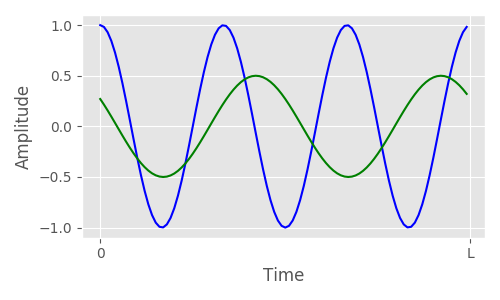
\includegraphics[scale = 0.8]{twoSinusoids.png}
	\label{fig:twoSines}
\end{figure}

Consider the two sinusoids in Figure 1, which will serve as a good example for illustrating orthogonality.  To 
take the inner product of these two sinusoids over some interval from 0 to some farther point in time $L$, 
one must sum the pointwise products of the amplitudes
for every instant in time between 0 and $L$.  The first pointwise product would be at $t = 0$ where $t$ 
represents time.  At that moment, the green sinusoid has an amplitude of about 0.25 and the blue sinusoid has
an amplitude of 1.0.  The product of these two values would be $1.0 * 0.25 = 0.25$.  That constitutes the first pointwise product.
To calculate the sum of all the other pointwise products, we would need to do this same procedure for every value of $t$
between 0 and $L$.  That's an infinite number of points!  Fortunately, 
if we can express these sinusoids in the form $A\sin(2\pi ft + \phi)$, then
it becomes relatively trivial with calculus and we can show that the result is indeed 0! 

Any two sinusoids of different frequencies are orthogonal no matter their phase or amplitude.  A key caveat though
is that the duration over which we take the inner product must usually be infinite in order to make this claim.  In 
music though, we never deal with infinitely long sine waves.  Songs are made up of finite length sine waves.  We
can still have orthogonality for any two sine waves over some finite interval from 0 to $L$, but we must provide
the extra condition that the waves are \textbf{periodic} along that interval.  This is a crucial point and one that 
will be paramount for 
understanding the limitations of the Discrete Fourier Transform.  If we look back at Figure \ref{fig:twoSines}, 
we will see that 
both the blue and the green sinusoids start and end at the same place in their respective curve.  If this were not true,
we could \textbf{not} make the claim that these two sine waves were orthogonal along that interval.  

Two periodic sinusoids are also orthogonal even when we sample them.  This is important because we will
never deal with periodic continuous sinusoids in a computer like those found in Figure \ref{fig:twoSines}.  We will be 
dealing with sampled signals and sinusoids.  To illustrate and provide a little proof on concept, let's sample the
two sinusoids from Figure \ref{fig:twoSines}.  For ease, let's assume that $L = 1$ so we will sample for one second
from both the green and blue sinusoids.  If you look at Figure \ref{fig:twoSines}, we can see that the green sinusoid
completes two complete cycles over a period of 1 second.  Therefore, it has a frequency of 2Hz.  The blue sinusoid
completes three full cycles so it has a frequency of 3Hz.  We need to choose a sampling rate that will not cause aliasing
for these two signals.  Anything above 6Hz will suffice, so let's choose 8 Hz.  Figure \ref{fig:twoSinesPoints} shows 
where those samples lie on our two sinusoids.  The samples for the blue sinusoid are approximately $b[n] = [1, -0.707, 0, 0.707, -1, 0.707, 0, -0.707]$ and the samples for the green
sinusoid are $g[n] = [0.27, -0.421, -0.27, 0.421, 0.27, -0.421, -0.27, 0.421]$.  The inner
product of $b[n]$ and $g[n]$ is equal to (1 * 0.27) + (-0.707 * -0.421) + (0 * -0.27) + 
(0.707 * 0.421) + (-1 * 0.27) + (0.707 * -0.421) + (0 * -0.27) + (-0.707 * 0.421) = 0.
Indeed these two sinusoids are orthogonal even when sampled.

\begin{figure}[h]
	\caption{Two sinusoids that are periodic along the interval 0 to $L$.}
	\centering
	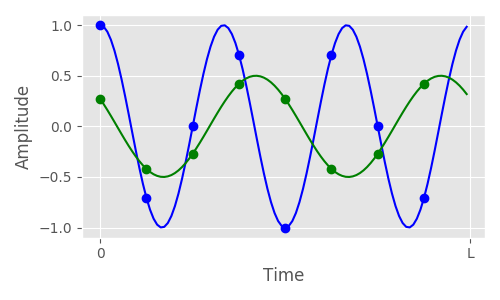
\includegraphics[scale = 0.8]{twoSinusoidsPoints.png}
	\label{fig:twoSinesPoints}
\end{figure}

Let's briefly summarize the conditions when two sinusoids of different frequencies
are orthogonal:

\begin{itemize}
	\item the two sinusoids are periodic along some time interval
	\item if sampled, the sample rate is greater than twice the frequency of both sinusoids
\end{itemize}

If you are curious more about how we can prove orthogonality and some of the issues with orthogonality for
continuous and discrete sinusoids, refer to Appendix A.

\section*{Probing for Sinusoids}

Ideally we would like some tool to be able to test whether a particular frequency is part
of some arbitrary signal.  We should be able to provide this tool some signal like a song
or speech and some frequency and our tool should be able to report back to use that either,
yes, this frequency is part of the signal or, no, the frequency is not part of the signal.
Figure \ref{fig:test} graphically depicts this procedure.  	Given such a tool, we could then 
iteratively test our signal for a whole range of frequencies
to construct the frequency domain of our signal.  This is exactly the procedure that the 
DFT performs.  It tests a signal for a whole range of frequencies to determine which are 
part of the signal and which are not.

\begin{figure}[h]
\caption{A sketch of the desired procedure for determining frequency in a signal.}
\centering
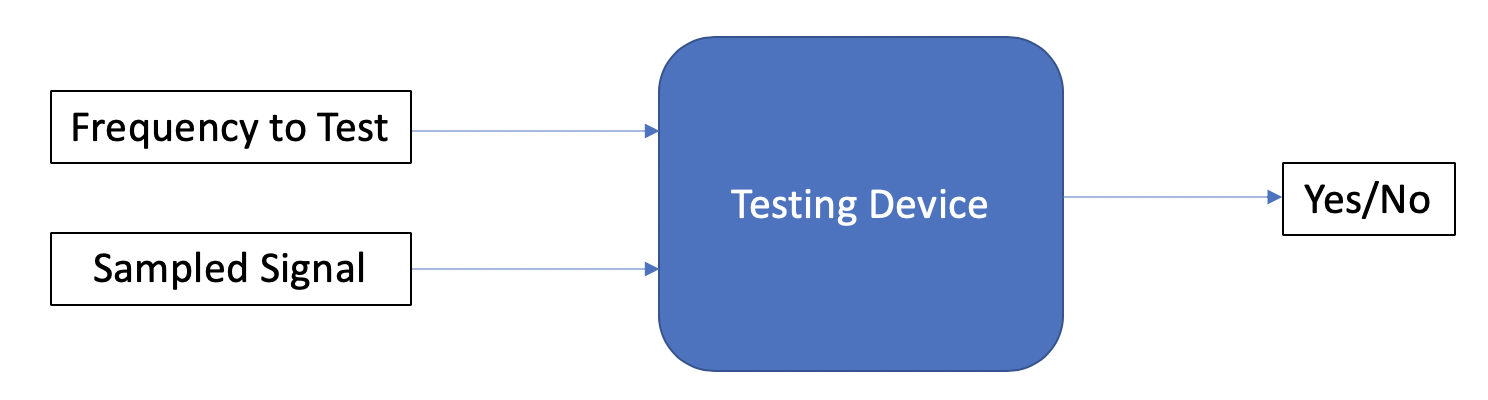
\includegraphics[scale = 0.4]{test.png}
\label{fig:test}
\end{figure}

Orthogonality will be our testing tool.  Let's imagine that our sampled signal was a simple
sinusoid of arbitrary frequency, phase, and amplitude.  Ahead of time, we do not know
anything about the sinusoid other than it is periodic along some time interval $L$.  Let's 
choose a frequency to test, say 100Hz, that we know is also periodic along $L$.  If we take
the inner product between the samples of the unknown sinusoid and the samples of 100Hz,
the result can provide some clues as to whether they are the same signal.  What do we know 
if the result is non-zero?  We can definitively conclude that they are the same frequency because
all periodic sinusoids of different frequencies are orthogonal.  What do we know if the result is 
zero?  The easy conclusion is to say that they must be different frequencies.  But that would
be a mistake!  We have not said anything yet about the inner product of two sinusoids of the
\textbf{same} frequency.  As it turns out, the inner product will almost always be non-zero 
unless the two sinusoids are out of phase by $\pi/2$.  So an inner product of zero almost
always means that the two sinusoids are of different frequency but not definitively.

	The inner product then is almost the perfect tool to help us distinguish between two
periodic frequencies.  Unfortunately, the pesky phase issue of $\pi/2$ for two sinusoids of 
the same frequency throws a wrench into the system.  In the next section, we will look at a way
to correct this problem.  But for now, let's assume that the inner product can perfectly distinguish
between the frequencies of two sinusoids.  

	We have shown how orthogonality can work as our testing tool for Figure \ref{fig:test} when
our signal is a sinusoid.  But rarely would our signal ever be just a simple sinusoid.  How can
we apply the inner product to an arbitrary signal like a song?  Recall that
any song, speech, soundscape, or any other kind of audio can be broken down into a sum of sinusoids.

$$A_1\sin(2\pi f_1 t + \phi_1) + A_2\sin(2 \pi f_2 t + \phi_2) + A_3\sin(2 \pi f_3 t + \phi_3) + ...$$

It turns out that the inner product is distributive.  So the inner product of some arbitrary signal applies
to each sinusoidal element that composes the signal.  The term ``distributive" in mathematics applies
to many different operations.  For example, we know from alebgra that the distributive property of 
multiplication over addition means that $x * (y + z) = x * y + x * z$.  We see that the multiplication operator can apply
to each individual component and the result is just the same.  If we have an arbitrary signal $x$ and another
arbitrary signal composed of components $y$ and $z$, then the distributive property for inner products 
means that  $\langle x, y + z \rangle = \langle x, y \rangle + \langle x, z \rangle$.  We will not spend any
time proving this truth here.  But it is actually not too difficult to do so.  The inner product is simply a
series of multiplications and additions.  So with some clever rearranging of terms, we can show that 
the distributive property is true for inner products.  

This is a wonderful result because we know now that when the inner product of some test frequency is 
applied to some arbitrary signal composed of sinusoids, the result is equivalent to the inner product of
our test frequency with each sinusoidal component.  We just analyzed the meaning of the inner product
of two sinusoids.  Anything that is non-zero means that two sinusoids are the same frequency.  Anything
zero is \textbf{almost} always means the two sinusoids are of different frequency.  Therefore, a non-zero result
of the inner product of some test frequency with an arbitrary signal means that the frequency is a part of that
signal.  A result of zero means that the frequency is likely not a part of the signal.  So the inner product
is our tool to implement Figure \ref{fig:test}.  

\begin{figure}[h]
	\caption{A realization of the desired procedure for determining frequency in a signal.}
	\centering
	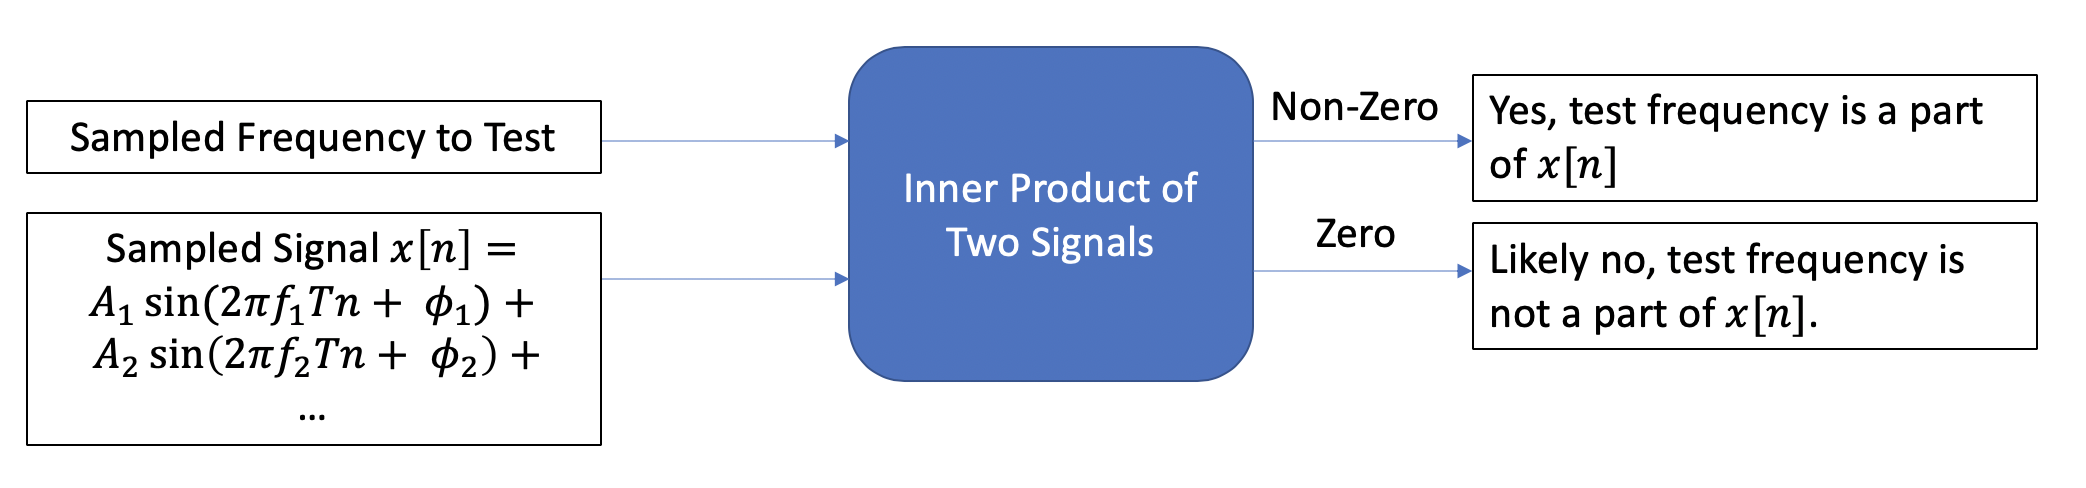
\includegraphics[scale = 0.4]{testImplemented.png}
	\label{fig:testImplemented}
\end{figure}

Figure \ref{fig:testImplemented} summarizes our methodology for implementing Figure \ref{fig:test}.  The inner
product is a tool that can distinguish whether two sinusoids are the same frequency with near certainty.  The next
section will show a way to make it foolproof.  Because the inner product is distributive, when it is applied to an
arbitrary signal and some test sinusoid, the inner product of the test with each sinusoidal component of different
frequency will be zero.  If any of the frequency components match our test frequency,  we will likely get a non-zero
result indicating that the test frequency is present in our signal.  Again, our test mechanism depicted in 
Figure \ref{fig:testImplemented} only works under the condition that the test frequency and the sampled signal
are periodic along the same interval.  

\section*{The Pesky $\pi/2$ Problem}

We know that the inner product of two sinusoids at different frequencies is always zero, assuming that the
sinusoids are periodic over some interval $L$.  However, that is not the $\textbf{only}$ way two sinusoids are
orthogonal.  It turns out that the inner product of two sinusoids of the $\textbf{same}$ frequency is zero when 
the sinusoids are separated by a phase of $\pi/2$.  This is a problem if we want to use the inner product to
test the similarity of two frequencies.  We do not want the inner product to be zero when the frequencies are the
same.  That should be reserved for different frequencies. 

How can we ensure that we get a non-zero inner product for sinusoids of the same frequency?  The answer:
take \textbf{two} inner products.  Suppose we have some test frequency and some signal and we would like to 
know whether that test frequency is a part of the signal just as described in Figure \ref{fig:test}.  If we take
the inner product between the test frequency and the signal, we run the risk that the answer could be zero even
if the test frequency is a part of the signal.  But if we have two test sinusoids of the same frequency but with
different phases, then at least one of them will yield a non-zero inner product with the signal if the signal 
contains the frequency of the test sinusoid.  

It may not be readibly apparent why using two sinusoids makes any difference.  For simplicity, let us say the
two sinusoids are sine and cosine.  Sine and cosine are separated by a phase difference of $\pi/2$.  Can you
think of another sinusoid of the same frequency with a phase different of $\pi/2$ for \textbf{both} of them?
The answer is no.  A sinusoid that $\pi/2$ away from cosine is either a sine wave or $\pi$ radians away from
sine.  In either case, that sinusoid would have a non-zero inner product with sine.  Therefore, using two inner
products, one with sine and one with cosine, creates a wonderful system where a zero inner product from both
cosine and sine means the frequency is conclusively not a part of the signal.

\begin{figure}[h]
	\caption{Complete solution for testing frequency components of a signal.}
	\centering
	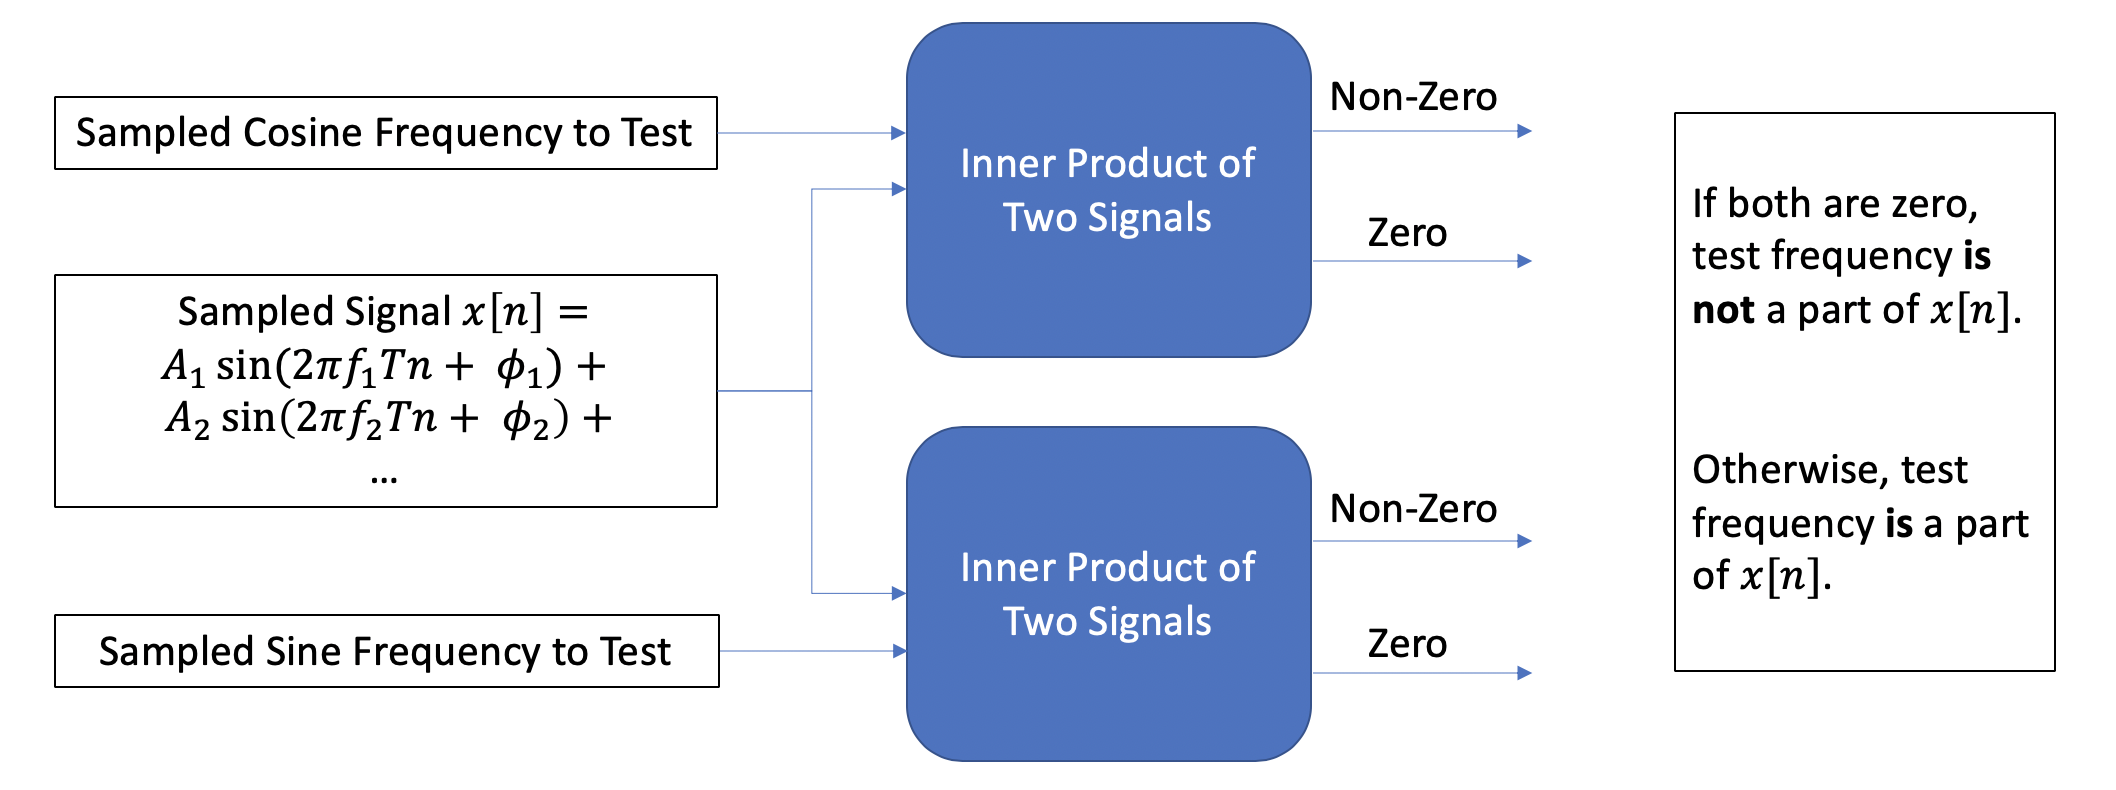
\includegraphics[scale = 0.4]{testComplete.png}
	\label{fig:testComplete}
\end{figure}

Figure \ref{fig:testComplete} shows our completed implementation of the testing mechanism outlined from
Figure \ref{fig:test}.  Note how we now need two sampled sinusoids: one cosine and one sine.  But now see
how an inner product of zero for both the sine test and cosine test definitively concludes that the frequency
is not a part of the signal.

If you are curious about how we can prove that $\pi/2$ is an issue, see Appendix B which walks through the math.

\section*{Imaginary Numbers}

Figure \ref{fig:testComplete} shows how we need to take the inner product of our signal with both a cosine and
sine wave to test whether a frequency is present in some signal.  Therefore, we will have two results, one for
each inner product.  It's a little cumbersome in math to express two separate results from some operation.  
Generally, if we compute something like $\sin(\pi/2)$, it yields a single numerical result.  

One way to do this would be to use vectors.  As we discussed above, vectors store a sequence of data and we
could put the result from the first inner product in the first slot of the vector and the second inner product in 
the second slot.  This would work perfectly well.  But there actually is a better solution: complex numbers.
Perhaps you have encountered complex numbers somewhere in your mathematical training.  Complex numbers
come in the form $a + bi$ where $i$ is called the imaginary unit or number and is defined as $i^2 = -1$.  Already,
this feels perilous on some level.  Why are we using complex numbers for audio signals?  There is nothing
``imaginary" about an audio signal, sine wave, or cosine wave.  So why use them?

In general, complex numbers are important mathematical tools for solving problems in mathematics, engineering and
the physical sciences.  This includes signals.  In fact, complex numbers are just as ``real" as say negative numbers.
It's hard to find a physical analogy to negative numbers.  We cannot pick up -4 rocks, for example.  Yet, we 
accept negative numbers because they allow us to work more easily with operators like subtraction.  Complex
numbers are similar.  They are a mathematical tool that allows us to solve problems we would not otherwise be
able to solve.  For our purposes, they serve a similar role to vectors.  When we have a number like $a + bi$, we
separate the real component $a$ from the imaginary component $b$.  You cannot add $a$ and $b$.  They are treated
as separate and distinct units.  We could very well use a complex number to express the number of apples and 
oranges.  Perhaps the real component represents the number of apples and the imaginary component represents
the number of oranges.  Then, to express that I have 3 apples and 4 oranges, I could write that as a single number
$3 + 4i$.  So one way to view a complex number is simply as a single number that has two distinct parts.  This
is what we need.  We can use the real component to hold the result of one inner product and the complex 
component to hold the other.

Complex numbers have one final important property that make them the ideal choice for our problem.  The great 
mathematician, Leonhard Euler, discovered one of the fundamental mathematical equations
that relates numbers such as $i$, $e$ and $\sin$ and $\cos$.  It is called Euler's formula:

\begin{equation}
\label{eq:euler}
e^{ix} = \cos(x) + i\sin(x)
\end{equation}

This is one of the most remarkable equations in all of mathematics.  The key takeaway is that we can use
a complex exponential to express both a real cosine term and an imaginary sine term.  Again there is
nothing ``imaginary" about the sine wave.  The complex exponential can simply be expressed as two 
\textbf{separate} sinusoids.  Fortuitously, a complex exponential is just what we need for our current
problem.  Remember we want to take the inner product of a signal with a cosine and sine wave, and we want to 
keep the results separate.  All we need to do then is to take the inner product of our signal with a complex
exponential.  For example, if we have a signal $x[n]$ and
we want to test it for frequency $f_{test}$, we can compute $\langle x[n], e^{2\pi f_{test}i}\rangle$.  This
notation says to take the inner product with the real cosine term of frequency $f_{test}$ and the inner
product with imaginary sine term of frequency $f_{test}$.  Because the real and imaginary numbers are kept
separate, we will get an answer of the form $a + bi$ where $a$ is the result of the inner product with cosine
and $b$ is the result of the inner product with sine. 

For digital signal processing, we will sometimes see Euler's formula express with a different variable $\omega$ which
stands for angular frequency.  Angular frequency is related to frequency by the equation $\omega = 2\pi f$.  So
we can rewrite Equation \ref{eq:euler} as $e^{i\omega} = \cos(\omega) + i\sin(\omega)$ or 
$e^{2\pi fi} = \cos(2 \pi f) + i\sin(2\pi f)$.  This better expresses the relationship between the frequency of the
sinusoids and the complex exponential.

Figure \ref{fig:testComplex} shows the updated version of our procedure for calculating the inner product.

\begin{figure}[h]
	\caption{Complete solution using complex exponentials.}
	\centering
	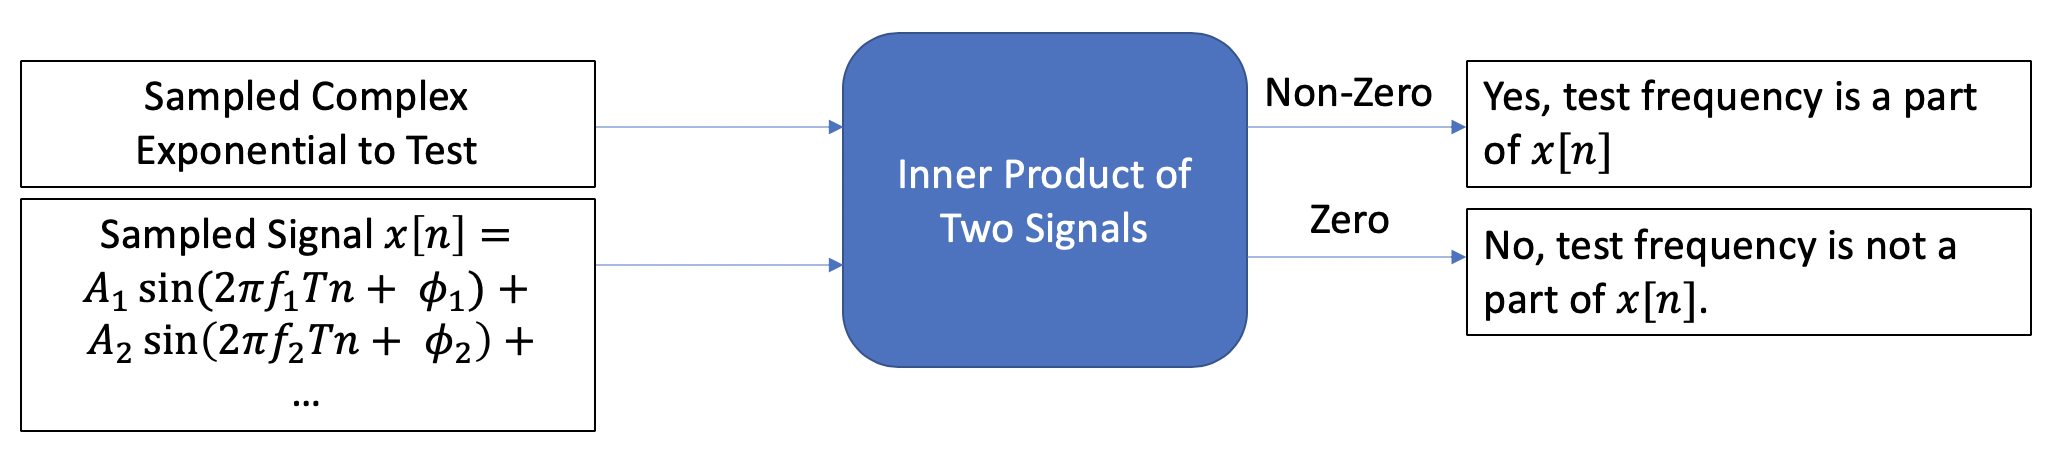
\includegraphics[scale = 0.4]{testComplex.png}
	\label{fig:testComplex}
\end{figure}

It is important to understand that Figure \ref{fig:testComplex} is no different from Figure \ref{fig:testComplete}.  
The inner product in Figure \ref{fig:testComplex} produces two inner products stored in the real and imaginary
components, respectively.  Those are the same inner products calculated in Figure \ref{fig:testComplete}.  If
both the real and imaginary component are zero then we know the test frequency is not a part of our signal
$x[n]$.

Unrelated to the issue of inner products, Euler's
formula also allows us to translate back and forth between sinusoids like sine and cosine and exponentials.
Exponentials are much easier to work with and allows us to quickly prove equations like trigonometric identities
that would be much harder if we simply had to work with just sine and cosine.  In general, if you plan to learn
more about digital signal processing, you will need to get comfortable with complex exponentials.

\textbf{**NEED TO MENTION ABOUT NEGATIVE AND SAY -SIN**}
	\section*{The Discrete Fourier Transform}

\subsection*{The DFT Equation}

We now have all the necessary knowledge to understand how the Discrete Fourier Transform works.  In fact, we
have essentially walked through most of it during our discussion of orthogonality and the inner product.  Before
I present the equation, remember that the DFT takes a finite number of samples and produces a finite frequency
spectrum.  The DFT makes an important assumption about those samples: \textbf{the samples contain an integer number 
of periods from some periodic signal}.  If the signal is periodic, then we know it can be represented as a sum of
harmonic sinusoids.  Therefore, we only need to test our signal for the harmonics instead of the entire frequency
spectrum.  This is tremendously important because we need to generate a finite frequency spectrum.  Furthermore,
assuming we have filtered out any frequency components above the Nyquist frequency, we only need to test harmonics
up to the Nyquist frequency.  The fundamental frequency of the harmonics is simply the duration represented
by the samples.  


Here is the equation for the DFT below:

\begin{equation}
\label{eq:dft}
X_k = \sum_{n = 0}^{N - 1}x[n] \cdot e^{-i\frac{2\pi}{N}kn}
\end{equation}

There is a lot to unpack here.  At a high level $X_k$ represents how much of some frequency we have in
some signal $x[n]$.  $X_k$ is a complex number and is the result of the inner product of our signal $x[n]$
and some test frequency denoted by the complex exponential $e^{-i\frac{2\pi}{N}kn}$.  If $X_k$ is zero, then
we know we do not have that frequency in $x[n]$.  If $X_k$ is non-zero, then we do have some amount of 
that frequency in $x[n]$.  

The DFT equation is just a mathematical description of the procedure described 
in Figure \ref{fig:testComplex}.  Importantly, \textbf{the equation for the DFT tests only one frequency.}  
$X_k$ is the result of just one test.  To build the entire frequency spectrum for an audio signal, we would
need to use the DFT equation multiple times.

Noticeably absent though from Equation \ref{eq:dft} is any mention of frequency, usually described with the
variable $f$.  Understand that the DFT is in fact calculating the inner product of the signal $x[n]$ with some
 frequency.  However, we cannot determine the frequency without knowing the sampling rate.  This is
 true if we look at any sequence of samples including those operated on by the DFT.
Take a sequence of samples from a simple sine wave.  We actually cannot make any
claims about the frequency of that sinusoid.  We need to know how fast those samples will be played back.  
 The faster the playback, then the higher the frequency.  Similarly, the slower the playback, then the lower
 the frequency.  Frequency can only be determined by the combination 
 of a sequence of samples in conjunction with a sampling rate, usually notated as $f_s$.  With the DFT, we
 make no assumptions about the sampling rate of the signal $x[n]$.  We treat $x[n]$ as just a sequence of
 samples and we test every sinusoid that could be periodic along that sequence of samples.

Remember orthogonality for finite sinusoids only holds for periodic sinusoids.  A sinusoid is periodic if it
completes an integer number of cycles across some period. 
In the DFT, that period is the number of samples of our audio signal $x[n]$ denoted by $N$. 
The variable $k$ denotes
the number of complete cycles that our testing sinusoid completes and specifies a harmonic
to test against $x[n]$.  If we know the sample rate $f_s$, we
can determine the frequency of the sinusoid we are testing using $k$ and $N$.  The sample rate is a ratio of
the number of samples taken per second.  If we divide the sample rate by $N$, we can calculate how many 
periods of $N$ it takes to span one second of time.  For example if $f_s = 1000$Hz and $N = 250$, then
$f_s/N = 4$ tells us that four cycles of $N$ constitutes one second of time.  If we know that our testing sinusoid
completes $k$ cycles over those $N$ samples, then it must complete $k \cdot f_s/N$ cycles per second.  This is
the frequency of the testing sinusoid.  Therefore, we can state that 

\begin{equation}
	\label{eq:freq}
	f = \frac{k}{N}f_s
\end{equation} 

\noindent Once we have the sampling rate, we know the
frequency represented by $X_k$.  In fact, you can see in the complex sinusoid
all the components for determing frequency (i.e., $\frac{k}{N}$) except the sampling rate.  
	
	Perhaps
you may be wondering why the sample rate is simply not included in the DFT equation.  That's a reasonable 
question and would make sense in the domain of audio.  In fact, we could write a variation of the DFT equation
that takes into account the sample rate of our signal by rearranging Equation \ref{eq:freq} and substituting it
into the DFT equation from Equation \ref{eq:dft}.

\begin{equation}
\label{eq:dftFS}
	X_f = \sum_{n = 0}^{N - 1}x[n] \cdot e^{-i2\pi \frac{f}{f_s}n}
\end{equation}

\noindent Here we take the same inner product of $x[n]$ with some complex sinusoid of frequency $f$ and known sample
rate $f_s$.  It is easy to see that this new variation is equivalent to Equation \ref{eq:dft} by the fact that 
$f = \frac{k}{N}f_s$.  However, if you were to use the version of the DFT from Equation \ref{eq:dftFS}, you
would need to be sure that the frequencies you tested were in fact periodic along the interval $N$.  While Equation
\ref{eq:dftFS} may translate the standard DFT equation to the variables of $f$ and $f_s$ with which you are likely
more comfortable, it becomes much less obvious what frequencies actually do complete an integer number
of cycles along $N$.  That is the purpose of the variable $k$ and why Equation \ref{eq:dft} is actually the easier
way to view the computation of the DFT.  It is also very little work to figure out the frequency with 
$f = \frac{k}{N}f_s$.

Below summarizes the meaning of each variable in the DFT equation.

\begin{itemize}
	\item $x[n]$: the signal
	\item $n$: the indexing variable
	\item $X_k$: a complex number that is the result of the inner product of $x[n]$ and a complex sinusoid
	\item $k$: the number of complete cycles our testing complex sinusoid completes
	\item $N$: the number of samples of our signal $x[n]$
	\item Frequency can be determined if the sampling rate is known by using $f = \frac{k}{N}f_s$
\end{itemize}

\subsection*{A Simple Example}

Let us use a simple example to illustrate the DFT equation.  Suppose
we have samples drawn from the following signal $x = 0.5\cos(2\pi t + \pi) + 0.25\cos(4\pi t - 1)$.  The signal
$x$ contains two sinusoids of frequency 1Hz and 2Hz, respectively, with differing phases and amplitudes.  
Let us say we
were to draw eight samples ($N = 8$) from $x$ at a sampling rate of 8Hz for ease.  Here are those samples below:

$$x[n] = [-0.3649, -0.1432, -0.1351, 0.1432, 0.6351, 0.5639, -0.1351, -0.5639]$$

Now let us use the DFT equation to check whether $x[n]$ contains the frequency 2Hz.  We 
of course know that it does but let us ensure that the DFT returns a non-zero value.  We
need to first figure out what $k$ should be.  We can simply solve using $f = \frac{k}{N}f_s$ and determine that
for $f = 2$, we should use $k = 2$.  Plugging in our values for $k$ and $N$ into Equation \ref{eq:dft}, we now 
need to compute the following:

$$X_2 = \sum_{n = 0}^{7}x[n] \cdot e^{-i\frac{\pi}{2}n}$$

\noindent Unfortunately, we cannot just simply plug this into our normal calculators and figure out what $X_2$ is.  The complex exponential needs to be converted into its sinusoidal form using Euler's formula as shown in Equation
 \ref{eq:euler}.  So let us rewrite that now:

$$X_2 = \sum_{n = 0}^{7}x[n] \cdot (\cos{(-\frac{\pi}{2}n)} +  i\sin(-\frac{\pi}{2}n)) = 
\sum_{n = 0}^{7}x[n]\cos{(-\frac{\pi}{2}n)} + i\sum_{n = 0}^{7}x[n]\sin(-\frac{\pi}{2}n))$$

\noindent Let us calculate each summation independently.  The left summation is the real part of the complex number $X_2$
and the right summation is the imaginary part.  

\begin{align*}
	\sum_{n = 0}^{7}x[n]\cos{(-\frac{\pi}{2}n)} =  & (x[0] \cdot 1) + (x[1] \cdot 0) + (x[2] \cdot -1) + (x[3] \cdot 0)\\
	& + (x[4] \cdot 1) + (x[5] \cdot 0) + (x[6] \cdot -1) + (x[7] \cdot 0)\\
	=  & x[0] - x[2] + x[4] - x[6] \\
	=  & -0.3649 - (-0.1351) + 0.6351 - (-0.1351) \\
	= & 0.5404
\end{align*}

Half of the result trivially goes away because many of those samples are multiplied by zero.  The bracket notation
$x[1]$, for example, simply means to use the first sample from $x[n]$.  Note that we count starting from index zero
in this notation so $x[1] = -0.1432$ and not $-0.3649$.  Using the same procedure, we can calculate
the imaginary summation as well.  That result is $-0.8415i$.  Therefore, the value of 
$X_2$ is $0.5404 - 0.8415i$.  Note that $X_2$ is non-zero!  Therefore we can see that the frequency 2Hz is
indeed part of our signal as it should be.

If we want to test whether 3Hz is a part of $x[n]$, then we can calculate the DFT with the appropriate $k$ for
3Hz which also happens to be 3.  Using the same procedure, we would find that $X_3 = 0 + 0i$.  $X_3$ is
zero, meaning that 3Hz is not part of $x[n]$ as expected.  Of course, we will almost always be using the
DFT on unknown signals for $x[n]$.  But as this small example illustrates, the DFT can let us test to see 
whether a periodic sinusoid is part of our periodic signal.

\subsection*{Reconstructing Amplitude and Phase}

While the DFT can tell us whether a certain frequency is part of some signal, it can do even better.  The complex
number $X_k$ can be used to reconstruct the amplitude and phase of the frequency as well.  Let us assume that
$x[n] = A\cos(2\pi f Tn + \phi)$ and that $x[n]$ is periodic along the interval
 $N$.\footnote{We could very well assumed a sinusoid of the form $A\sin(2\pi fTN + \phi)$ instead of using a 
cosine.  It certainly makes no mathematical difference as a sine wave and cosine wave are only differentiated
by their phase.  It will be nicer mathematically if we think about it as a cosine wave.  The corresponding
$X_k$ would have a complex number of the form $	X_k = \frac{AN\sin(\phi)}{2} - \frac{AN\cos(\phi)}{2}i$. While this is perfectly valid, the careful reader will note that the angle or argument of the complex number
does not match $\phi$ as it does in the cosine form.  The cosine form presents a nice convenience.}  
Therefore, we can also write the sinusoid in the form $A\cos(2 \pi \frac{k}{N} n + \phi)$ using Equation \ref{eq:freq}.  The
latter form matches nicely with $X_k$ because the subscript $k$ from $X_k$ is the same $k$ in 
$A\cos(2 \pi \frac{k}{N} n + \phi)$.  When we take the DFT for $x[n]$,  the complex number will be of the form
shown in Equation \ref{eq:complexNumber}.

\begin{equation}
	\label{eq:complexNumber}
	X_k = \frac{AN\cos(\phi)}{2} + \frac{AN\sin(\phi)}{2}i
\end{equation}

 In some notations for complex numbers, the real part and imaginary parts of a complex number are referred to
 using the following operators: $\RE()$ and $\IM()$, respectively.  If the imaginary number $z = 3 + 4i$, then
 $\RE(z) = 3$ and $\IM(z) = 4$.  The symbols themselve may seem cumbersome but they are
 simply a convenience for referring to the components of an imaginary number.  Therefore, we can say
 based on Equation \ref{eq:complexNumber} that $\RE(X_k) = \frac{AN\cos(\phi)}{2}$ and $\IM(X_k) = 
 \frac{AN\sin(\phi)}{2}$.  Given Equation \ref{eq:complexNumber} and our new notation, the amplitude $A$ 
 can be dervied from $X_k$ as follows:


\begin{equation}
\label{eq:amplitude}
	A = \frac{2}{N}\sqrt{(\RE(X_k))^2 + (\IM(X_k))^2}
\end{equation}

Recalling our example above, let us reconstruct the amplitude from $X_2 = 0.5404 - 0.8415i$.  Plug in 
the real and imaginary components to Equation \ref{eq:amplitude}.  We then get 
$A = \frac{2}{8}\sqrt{(0.5404)^2 + (-0.8415)^2} = 0.25$.  If we look back at the original signal $x =
0.5\cos(2\pi t + \pi) + 0.25\sin(4\pi t - 1)$, you will see that the sinusoid with frequency 2Hz does indeed
have an amplitude of 0.25.  For those familiar with complex numbers, Equation \ref{eq:amplitude} looks 
remarkably close to the formula for the magnitude of a complex number.  The magnitude of complex number
$z$ is $\sqrt{(\RE(z))^2 + (\IM(z))^2}$.  The only difference then is a scaling factor of $2/N$.  Equation \ref{eq:amplitude}
is sometimes referred to as the ``normalized magnitude".

Similarly, we can also use $X_k$ to reconstruct the phase $\phi$ of the sinusoid.  Equation \ref{eq:phase}
shows the formula for doing so.

\begin{equation}
\label{eq:phase}
\phi = \tan^{-1}\bigg(\frac{\IM{(X_k)}}{\RE{(X_k)}}\bigg)
\end{equation}

\noindent From the same example, if we compute $\tan^{-1}(\frac{-0.8415}{0.5404})$, we get $-1$ which is indeed the
phase of $0.25\sin(4\pi t - 1)$.  One needs to be careful when using the inverse tan function with computers
or calculators.  The sign of the real and imaginary part indicates which quadrant the phase will be located.  Most
computers and calculators however wrap the phase between $-\frac{\pi}{2}$ and $\frac{\pi}{2}$.  Some software
like Matlab and others offer a special function that accounts for the sign of the numerator and denominator.  It is sometimes referred to as ``atan2".  It is fine to use either but you may need to correct some phases by 
hand if your calculator wraps the phase between $-\frac{\pi}{2}$ and $\frac{\pi}{2}$.

Equations \ref{eq:complexNumber}, \ref{eq:amplitude}, and \ref{eq:phase} apply to nearly all $X_k$. 
The exceptions are when $k/N$
is a multiple of $\frac{1}{2}$, corresponding to $k = N/2$ (i.e., the Nyquist frequency) and $k = 0$ 
(sometimes termed the DC offset in electronics).\footnote{DC offset refers to how far away the average of a signal
deviates from zero.  It is not a component of the signal that contributes to pitch.}  In these 
instances, the complex number $X_k$ cannot be used to recover the original amplitude and phase because
$X_k = AN\cos{(\phi)} + 0i$.  Since the imaginary component is zero, we do not know
what proportion of $A$ and $\phi$ contribute to the real component of $X_k$.  For the DC offset, this is not an issue.
A sinusoid with $k = 0$ is simply of the form $A\cos(\phi)$ and evaluates to a scalar.  It does not matter
what proportion of amplitude and phase contribute to the scalar, simply the value of the scalar itself.  The
Nyquist frequency  similarly does not pose a problem.  We do not expect to have
any frequency component at the Nyquist frequency if we have properly filtered our signal to prevent aliasing.

\subsection*{Frequency Bins}

The DFT equation from Equation \ref{eq:dft} only calculates the inner product of $x[n]$ and one
frequency.  However, we want to calculate the DFT for numerous frequencies.  Remember that
frequency is not explicitly stated in the DFT equation but rather implied by $k$ in conjunction with the 
sampling rate.  To flesh out the full frequency spectrum, $X_k$ is calculated for every value of $k$ from 0  to $N - 1$. 
Each calculation of $X_k$ is sometimes referred to as a frequency bin. 
A value of $k = 0$
calculates how much DC offset is in the signal (i.e., if the averages of the samples is something other than zero).
A value of $k = \frac{N}{2}$ tests for presence of the Nyquist frequency defined as half the sampling rate.  We do
not need to test for values of $k \geq N$ because the values of the DFT repeat.
You can test this yourself as $X_0 = X_N$ and $X_1 = X_{N + 1}$ and so on.

\begin{figure}[h] 
	\caption{A table of the DFT results from samples of $0.5\cos(2\pi t + \pi) + 0.25\cos(4\pi t - 1)$}
	\label{fig:dftTable}
	\begin{center}
		\begin{tabular}{ |c|c|c|c|c|c|c| } 
			\hline
			k & Frequency (in Hz) & $X_k$ & Amplitude & Phase \\ 
			\hline
			0 & 0 & $0 + 0i$ & 0 & 0 \\ 
			1 & 1 & $-2 + 0i$ & 0.5 & $\pi$ \\
			2 & 2 & $0.5403 - 0.8415i$ &0.25 & -1 \\
			3 & 3 & $0 + 0i$& 0 & 0 \\
			4 & 4 & $0 + 0i$  & 0 & 0 \\
			5 & 5 & $0 + 0i$  & 0 & 0 \\
			6 & 6 & $0.5403 + 0.8145i$ & 0.25 & $1$ \\
			7 & 7 & $-2 + 0i$  & 0.5 & $-\pi$ \\
			\hline
		\end{tabular}
	\end{center}
	
\end{figure}

Figure \ref{fig:dftTable} shows a table of all the calculations from the DFT in the column labeled $X_k$.  For
convenience, the frequency of each bin is also given.  Because the number of samples equals the sampling rate,
$k$ is equivalent to frequency of the $k$th bin, but that will rarely be the case.  We generally deal with very high
sampling rates like 44.1kHz and smaller numbers of samples for the DFT.  To calculate the frequency of each
$X_k$, sometimes referred to as frequency bins, we simply compute $k\frac{f_s}{N}$.  You can see that in
our trivial example that $\frac{f_s}{N} = \frac{8}{8} = 1$ so the frequency of each bin is just $k$.

Figure \ref{fig:dftTable} also has  columns for amplitude and phase as calculated using Equations 
\ref{eq:amplitude} and \ref{eq:phase},
respectively.  We can see that for a frequency of 1Hz there exists
 a sinusoid of amplitude 0.5 and phase $\pi$ and for a frequency of 2Hz there exists a sinusoid of 
 amplitude 0.25 and phase $-1$.  As expected the samples for $x[n]$ were taken from a signal 
 matching the specifications of those two sinsusoids, namely $0.5\cos(2\pi t + \pi) + 0.25\cos(4\pi t - 1)$.
 
 We can also see that we seemingly have extra sinusoids in our frequency domain at 6Hz and 7Hz.  
 We can ignore these frequencies.  The DFT is symmetric about the Nyquist frequency so any 
 frequencies below the Nyquist frequency will appear above the Nyquist frequency.  This is simply
 a byproduct of the math used for the DFT.  We could have simply just calculated the frequency
 for bins $k = 0$ up to the Nyquist frequency.  However, the standard frequency domain computed
 by the DFT ranges from $k = 0$ to $N - 1$.  For audio signals, the upper half of the frequency
 domain is unimportant but for different signals it is.
 
\subsection*{Interpreting The Magnitude and Phase Spectra}

When we calculate the DFT,  we often display the magnitude and phase of each $X_k$ graphically.  Below
are two examples of the magnitude and phase spectrum of some signal $x[n]$ with sample rate $f_s = 256$Hz and
$N = 128$.  Let us see what we can deduce about the time domain form of the signal from these two spectrums.

\begin{figure}[h]
	\caption{The magnitude spectrum of $x[n]$ at $f_s = 256$ and $N = 128$}
	\label{fig:magnitudeGraph}
	\begin{center}
	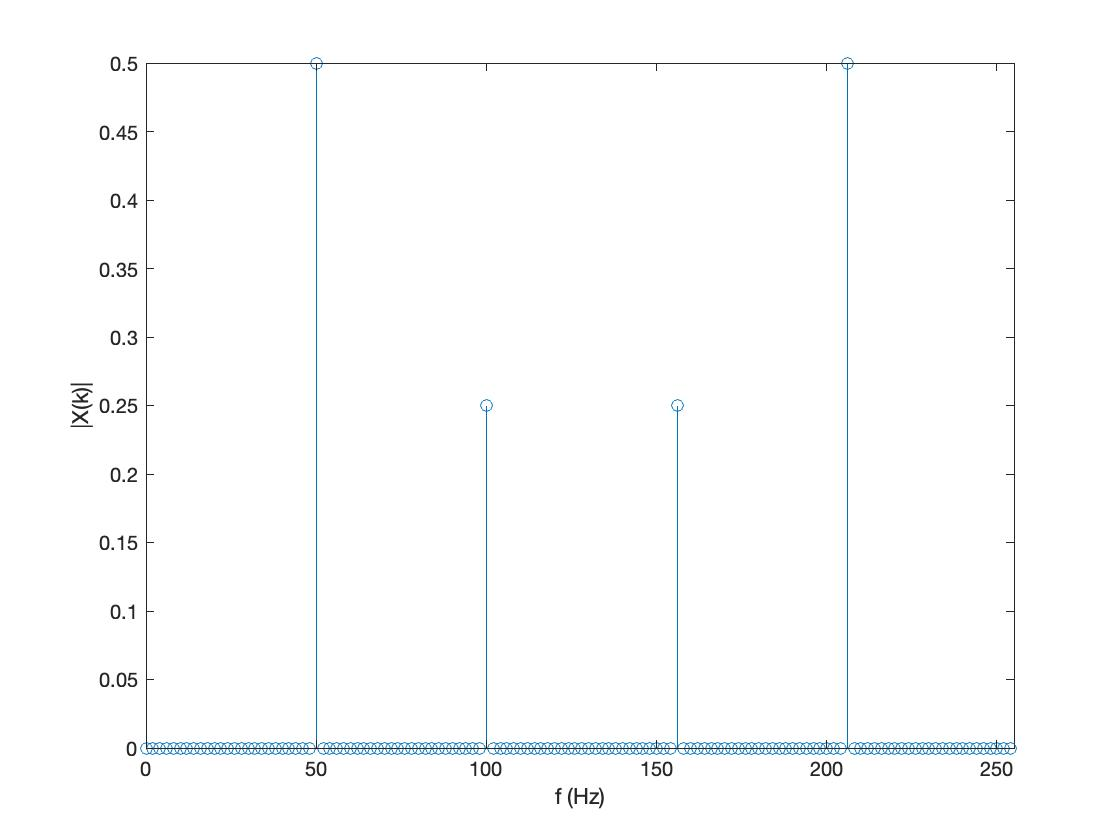
\includegraphics[scale = 0.3]{magnitude.jpg}
	\end{center}
\end{figure}

\begin{figure}[h]
	\caption{The phase spectrum of $x[n]$ at $f_s = 256$ and $N = 128$}
	\label{fig:phaseGraph}
	\begin{center}
		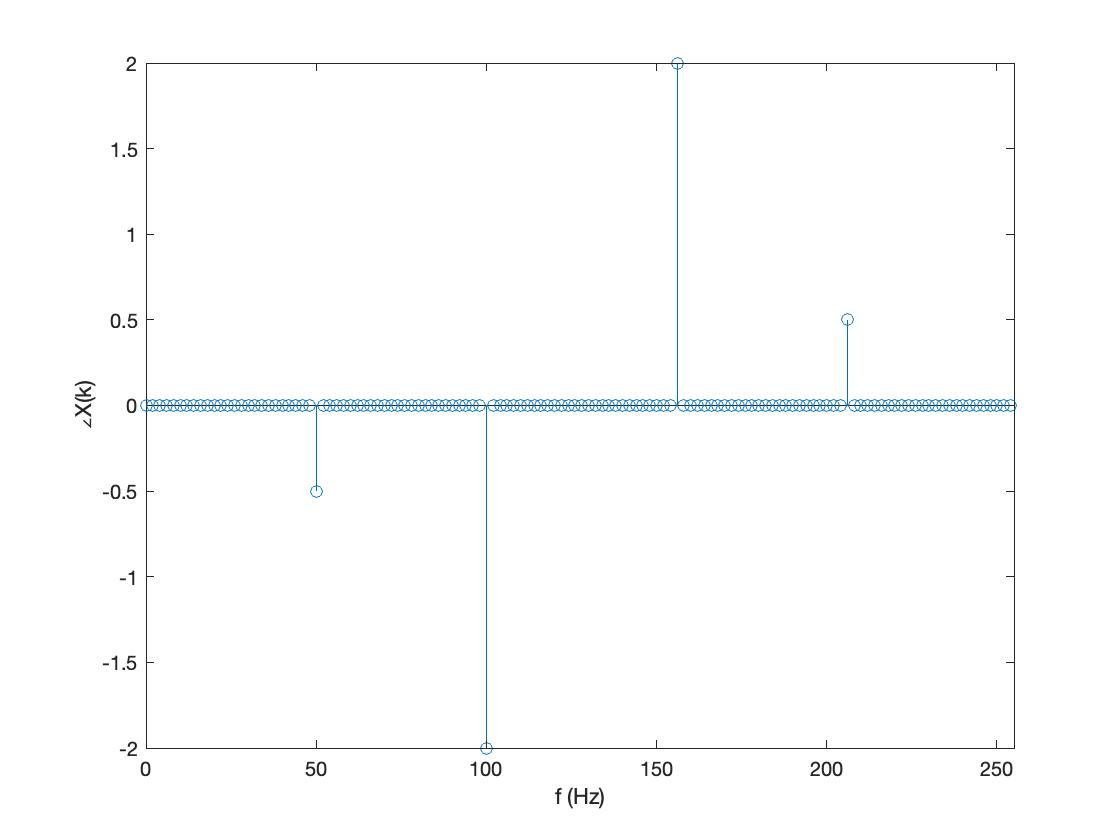
\includegraphics[scale = 0.3]{phase.jpg}
	\end{center}
\end{figure}

Figure \ref{fig:magnitudeGraph} shows the magnitude spectrum of $x[n]$.  Here we plot the magnitude of
each $X_k$.  Recall that the magnitude of a complex number $z$ is defined as $\sqrt{(\RE(z))^2 + (\IM(z))^2}$.
It is quite common to see plots of the magnitude spectrum
using simply the magnitude of each $X_k$.  To derive the amplitude of the original frequencies, we must multiply
each value in the figure by $2/N$ to match Equation \ref{eq:amplitude}.  
Alternatively, some magnitude spectrum are plotted on a decibel scale.  It is always important to
check how the magnitude spectrum is plotted as there are several variations.

	In Figure \ref{fig:magnitudeGraph}, we see four peaks in the graph.  We can conclude that there are four 
frequency components at frequencies 50Hz, 100Hz, 156Hz, and 206Hz.  
We can ignore the components of the spectrum above the Nyquist frequency of 128Hz. 
Therefore, we have two
sinusoidal components in $x[n]$: 50Hz at an amplitude of 0.5 and 100Hz at an amplitude of 0.25.  

Note the symmetry in the magnitude spectrum.  If we were to draw a straight line down the center of the 
magnitude spectrum at the Nyquist frequency, the left half and right half would be perfectly symmetrical.  
A fundamental property of the DFT is that when $x[n]$ is a real signal and does not include any complex
components, the two halves of the magnitude spectrum are symmetrical.  Because we are dealing solely 
with audio signals,
we always use the DFT with real signals and therefore will always have symmetry.  

Figure \ref{fig:phaseGraph} shows the phase spectrum of $x[n]$.  The phase spectrum of a signal plots
the argument of the complex number $X_k$.  Those familiar with complex numbers will note that
 the argument of a complex number is also calculated 
using Equation \ref{eq:phase}.  Thus, the argument of each $X_k$ is the same as the phase of
the frequency component, assuming we model the frequency component 
as a cosine wave.  As expected we see peaks at exactly 50Hz, 100Hz, 156Hz, and 206Hz.  Again, we can 
ignore the two frequencies above the Nyquist frequency.  We can see phases of $-0.5$ and $-2$ at 50Hz and 
100Hz, respectively.  Putting together the information from the magnitude and
phase spectrum, we can perfectly recreate the original signal: 
$x[n] = 0.5\cos(2\pi(50)t - 0.5) + 0.25\cos(2\pi(100)t - 2)$.

There is also symmetry in the phase spectrum as well.  Again if we were to draw a straight line vertically at
the Nyquist frequency and flip the signs of one of the halves, we would have two symmetrical halves.  Again
these symmetrical properties are true for all real signals $x[n]$ such as audio.

	\section*{Periodicity}

\subsection*{DFT Assumptions}

We have discussed at length how two sinusoids of different frequencies are orthogonal, assuming they
are both periodic along some interval.  This was a key assumption that allowed us to parse a signal into 
its various constituent frequencies.  Recall that any signal can be broken down into a summation of sinusoids,
and that the inner product is distributive.  
Therefore taking the inner product of some signal $x[n]$ with
a sinusoid $s$ is the same as taking the inner product of $s$ with each sinusoid that
constitutes $x[n]$.  Everything that we have learned so far has hinged on the assumption that all sinusoids, 
including the ones that make up $x[n]$, are periodic along that same interval of samples $N$.  

If you look back
at the small example from earlier, the signal $x[n]$ was composed of two sinusoids $0.5\sin(2\pi t + \pi)$
and $0.25\sin(4\pi t - 1)$, both of which are periodic over one second.  When we took the DFT of that signal,
we tested $x$ for frequencies of 0Hz, 1Hz, 2Hz, etc., all of which are also periodic over one second.  This
example was contrived to work perfectly within the assumptions of the DFT, namely that both $x[n]$ and
our testing frequencies were periodic over the number of samples from the signal.  

In the real world, we will rarely, if ever, be that lucky.  If we were to take a series of $N$ samples from a song
or a speech, it is very unlikely that the slice of audio would be periodic along $N$.  So what are we to do?  Is the
DFT somehow now unusable?  The answer is no.  But we do need to recalibrate our assumptions of what
it can and cannot do.  For one, the DFT cannot tell us all the frequencies
and their respective amplitudes and phases with complete precision for any signal.  
The DFT, however, can give us a good \textbf{estimate} of what frequencies are part of some signal.

For $x[n] = A\cos(2 \pi \frac{k}{N} n + \phi)$, we were able to show precisely what the value of
$X_k$ would be as shown in Equation \ref{eq:complexNumber}.  Though we did not show the derivation for 
that equation, it is similarly
based on the assumption that $x[n]$ is periodic along $N$.  Therefore,
we will not be able to use Equation \ref{eq:complexNumber} for aperiodic $x[n]$.  As a consequence, we 
cannot use Equation \ref{eq:amplitude} and 
Equation \ref{eq:phase} to recover the original amplitudes and phases
 as these are derived from Equation \ref{eq:complexNumber}.  Not all hope is lost
though.  We can still use the DFT to say plenty about the frequency spectrum of $x[n]$.  The magnitude of 
$X_k$ will give us a good estimate of the relative strength of the frequency components in the original 
signal as we will see shortly.  

Some of our conclusions will remain the same regardless of the periodicity of $x[n]$.  The symmetry we saw 
in the magnitude and phase spectrum still applies.  We shall also see that we can perfectly recover the 
original $x[n]$ regardless
of its periodicity using a technique called the Inverse Discrete Fourier Transform.

Though the DFT has shortcomings and does not give the complete picture of the frequency domain for
all $x[n]$, it is still incredibly powerful and useful.  We will still be able to gain a tremendous amount of
information about our signal and do some interesting spectral processing to create engaging audio effects.

\subsection*{DFT of an Aperiodic Sinusoid}

Let us consider what happens when we take the DFT of a signal that is not periodic along $N$.  For ease, let us
start with the simplest of signals, a sinusoid.  We will take $N = 32$ samples from a cosine wave 
that is not periodic along $N$.  The frequency of the cosine wave will be 2.7Hz with an amplitude of 0.5 and a phase of
2.  To get the samples, we can use $x[n] = 0.5\cos(2\pi (2.7)Tn + 2)$ and compute the values for 
$n = 0, 1, 2,...$ etc.
The sampling rate is 32Hz (and thus $T = 1/32$) 
which means we will produce frequency bins of 0Hz, 1Hz, 2Hz, etc.  Importantly, note that there is no frequency bin 
for 2.7Hz.  

\begin{figure}[h]
	\caption{The time domain, magnitude and phase spectra of $x[n] = 0.5\cos(2\pi (2.7)Tn + 2)$
	for $N = 32$ and $f_s = 32$Hz.}
	\label{fig:aperiodicGraph}
	\begin{center}
		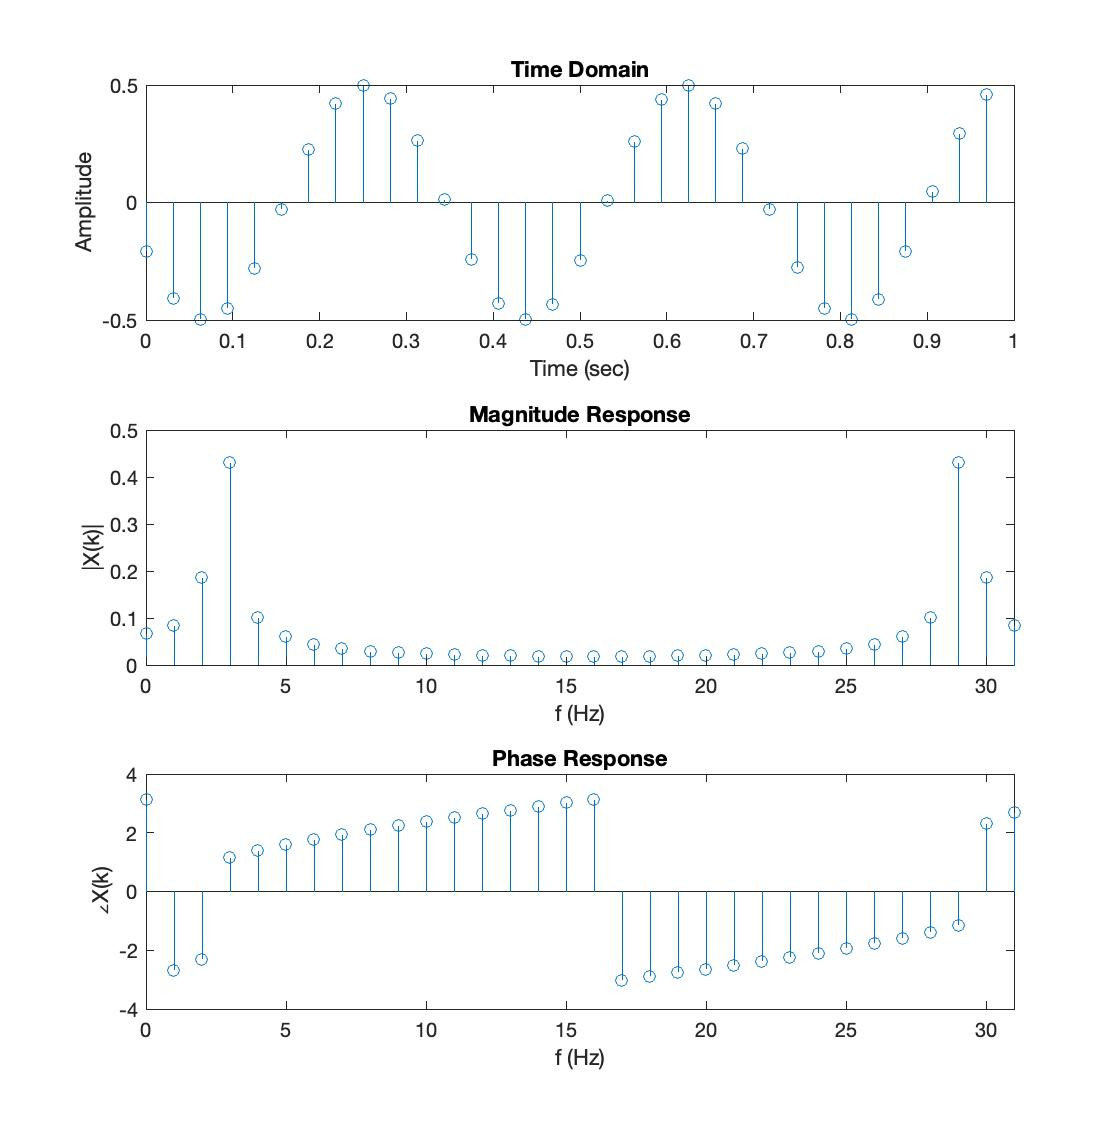
\includegraphics[scale = 0.3]{aperiodic.jpg}
	\end{center}
\end{figure}

Plotted in Figure \ref{fig:aperiodicGraph} is the magnitude and phase spectra of the original signal as well as its time 
domain representation.  Notice that the time domain clearly shows that $x[n]$ completes
two full cycles \textbf{plus} some fractional number of cycles.  After computing the DFT of $x[n]$, Figure 
\ref{fig:aperiodicGraph} shows the magnitude and phase spectra.
The magnitude spectrum was calculated by taking the magnitude of each complex number.  
If we look at the graph, we can see two peaks roughly between 2Hz and 3Hz
and between 29Hz and 30Hz.  We can also see the symmetry between the two halves if we split the magnitude spectrum
down the middle.  We can see that every frequency bin has some magnitude in it which might suggest that our original
signal was composed of 32 sinusoids of varying amplitudes.  But we know that is not the case.  There is just one at
2.7Hz.  We can, however, see ``activity" at 2.7Hz in the magnitude spectrum due to the vertical peak.  The other peak
is simply the mirror image of 2.7Hz above the Nyquist frequency.  We saw this symmetry occurred even with periodic
sinusoids.  So many of the same instincts that we derived in the context or periodic $x[n]$ hold true with aperiodic 
$x[n]$. 

How do we account though for positive magnitudes in all the bins?  This is a phenomenon called \textbf{spectral leakage}.  
We will always see peaks in the magnitude spectrum at the frequencies of $x[n]$ provided those frequencies have
sufficient amplitude.  Notice though that each frequency bin registers some level of magnitude.  Farther away from the 
peak, the magnitudes decrease but are still non-zero.  This is called ``spectral leakage".  It is important to understand
that we are not seeing multiple frequencies.  Rather we are seeing the effect of how one aperiodic component of $x[n]$
spreads out to all frequency bins.   

Can we recover the original amplitude of 0.5 from the magnitude spectrum?  The answer, in short, is no.  For one, we
would need to guess about where the apex of the peak was.  The peak is always centered at the frequency of each
component of $x[n]$.  It is hard to tell based on the magnitude spectrum though where exactly that is.  We can use
a process called interpolation to estimate the peak.  Even so, each frequency component of $x[n]$ spreads to each
adjacent bin.  Therefore, even if we could determine the peak, the magnitude at that location could be the product
of the spread of several different peaks.  Therefore, it will be impossible to reconstruct the original amplitude.  
Nevertheless we can get a good sense of the relative strength of each component.  Higher peaks represent stronger
frequency components; lower peaks represent weaker frequency components.

How can we interpret the phase spectrum?  Again we see a sudden change around 2Hz.  The phase spectrum shifts
drastically at the location moving from negative to positive.  It is hard though to see any relationship between the phase spectrum of $x[n]$ around 2.7Hz and the original phase.  In 
general, the phase spectrum of the DFT is more abstruse and difficult to parse.  Sometimes sudden shifts in the
phase spectrum are the result of the periodic nature of sinusoids.  Phases outside the range $+\pi$ to $-\pi$ get
wrapped back down to that range.  This can cause abrupt shifts in the phase spectrum.  We will not be spending
much time examining the phase spectrum as it usually is less important for musical applications. We shall see soon
though that there is a better way to interpret the phase spectrum.

\subsection*{The Periodicity of the DFT}

We have seen how the DFT responds to periodic and aperiodic sinusoids.  In this section, I would like to offer 
another perspective on the DFT.  We have learned that the DFT can accurately parse the frequencies of $x[n]$ if
$x[n]$ is periodic along those $N$ samples.  I should also state explicitly that the DFT \textbf{assumes} that
those $N$ samples are from a periodic function regardless of whether they are or not and that those $N$ samples
constitute a period from that periodic signal $x[n]$.  

If we look back at the time
domain representation of Figure \ref{fig:aperiodicGraph}, we can see a plot of the samples from the sinusoid of
2.7Hz.  The DFT assumes those $N$ samples make up one period of the periodic signal $x[n]$.  $x[n]$
is indeed periodic but those $N$ samples are not a period of $x[n]$.  One way to see what the DFT ``sees" is to
simply repeat those $N$ samples and look at the time domain representation of the sound.  The top plot in Figure
\ref{fig:basis} shows a plot of 2.7Hz with a smaller sampling period to highlight the disjointed transition when the samples
repeat.  Importantly, the DFT is parsing the frequencies of \textbf{this} signal and not the smoothly oscillating sinusoid 
from where the samples originated.  Another way, then,
to think about spectral leakage is that it is the distortion of the original waveform that occurs when we fail
to capture a complete period.

\begin{figure}[h]
	\caption{Periodicity of the DFT as shown through the time domain representation in the samples and the cosine basis}
	\label{fig:basis}
	\begin{center}
		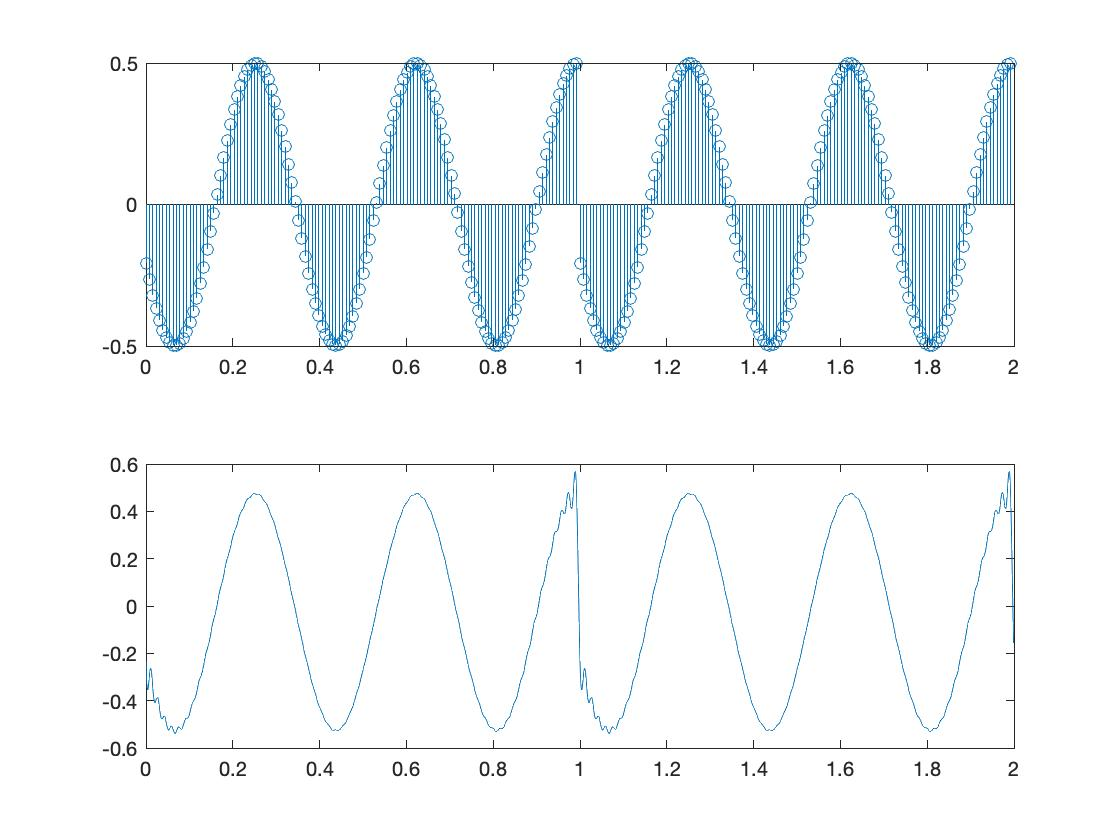
\includegraphics[scale = 0.3]{basis.jpg}
	\end{center}
\end{figure}

Consider again the N aperiodic samples from the sinusoid 2.7Hz. In that example,
we took a slice of $N = 32$ samples from $x[n] = 0.5\cos(2\pi (2.7)Tn + 2)$.  Nevertheless, the DFT still considered those $N$ samples to be periodic.  Again, the top plot in Figure \ref{fig:basis} shows how the DFT perceives the periodicity of that waveform.\footnote{
	Here though we have increased the number of samples and sampling rate 
	($N = 128$ and $f_s = 128$Hz) for higher resolution.
}
Because this distorted signal is periodic, we can represent it using a sum of harmonic sinusoids.  The bottom plot from Figure \ref{fig:basis} shows an approximation of that signal with a sum of harmonic cosine waves.  
How can we determine which cosine waves to sum?  From the DFT, of course!  
\textbf{Another interpretation of the
DFT is that it encodes the information to recreate the N periodic samples using a sum of harmonic cosine waves.}  
The frequencies
of the DFT bins form a harmonic series with a fundamental period equivalent to the time spanned by the $N$ samples.
Therefore, we can use $X_k$ to construct the amplitude and phase of each sinusoid.

The magnitude and phases we calculate for each frequency bin
can be used in conjunction with the frequency of each bin to construct a series of cosines waves that,
when summed, produce the approximation shown in the bottom plot from Figure \ref{fig:basis}.  For example,
the first frequency bin has a frequency of 0 where $X_0 = AN\cos(\phi)$. Remember we are interpreting the $N$ samples
as periodic, therefore we know $X_0 = AN\cos(\phi)$.  For subsequent $X_k$, we can rely on Equation \ref{eq:amplitude} and
\ref{eq:phase} to determine the amplitude and phase of each frequency bin.  For example, the second
 frequency bin has a frequency of 1Hz, a magnitude of 0.0696, and a phase of $-2.6026$.  If we plug those values into
 a cosine wave, we get $0.0696 * \cos(2 * \pi * (1) * t - 2.6026) = 0.0696\cos(2\pi t - 2.6026)$.  We can add this to
 $-0.0261$ to get the first two sinusoidal harmonics.  If we continued in this fashion with every frequency bin
 up to $k = N/2$, the Nyquist frequency, we get the approximation shown in the bottom plot from 
 Figure \ref{fig:basis}.  
 
 	In this interpretation of the DFT, we can see how both the phase and magnitude derive meaning.  We can think
 of the DFT as producing a series of harmonic cosine waves that get their specific parameters from the values in each
frequency bin.  We call these harmonic cosine waves a \textbf{basis}, and we \textbf{project} our original signal
$x[n]$ onto this basis.  This is the geometric interpretation of the DFT.  The terms ``projection" and ``basis" are 
mathematical terms.  One common ``basis" we all know is the coordinate axis system.  It is a space that allows us
to plot any 2D shape.  A series of harmonic cosine waves also form a basis.  It is a basis that allows us to 
plot or describe any periodic signal.  We can think of projection as a means to describe our original signal
 in terms of our basis (i.e., a sum of cosine waves).  But how exactly do we do this projection?  
 With the inner product.  The inner product, with which we started our duscussion of the DFT,
 is a means of projecting a signal onto a different basis such as the frequency domain.  Therefore, another way to
 view the DFT is that it takes a period of $N$ samples and projects them onto a set of harmonic sinusoids that
 approximate the waveform described by those $N$ samples.

	\section*{The DFT on Real-World Sounds}

\subsection*{The DFT on Audio}

So far we have used contrived examples to get a better understanding of how the DFT works on both periodic and
aperiodic samples.  Let us put it all together and examine an unknown piece of audio.  We will look at the magnitude
spectrum of the samples and draw some conclusions about the original audio file.  Later in this section, I
will reveal the origin of the audio file and we can reexamine our conclusions.  Figure \ref{fig:unknown} shows the 
time domain representation and magnitude spectrum of this signal.  We will ignore the phase spectrum as it
is difficult to glean meaningful information from the signal.

\begin{figure}[h]
	\caption{The time domain and magnitude spectrum plots of an unknown audio signal}
	\label{fig:unknown}
	\begin{center}
		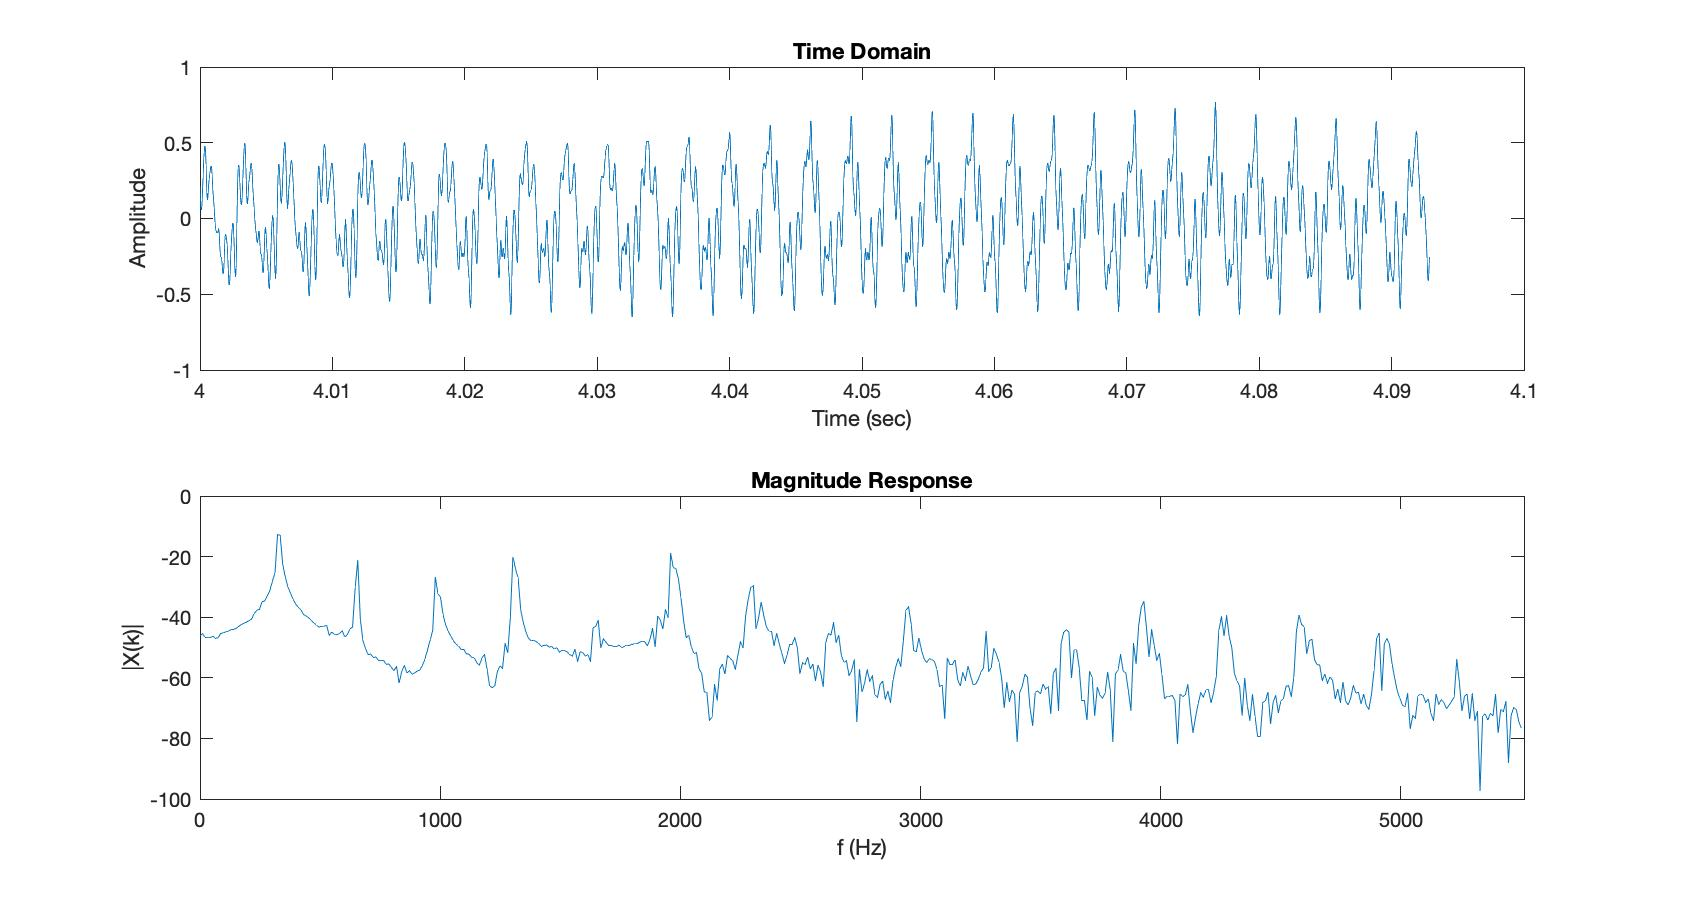
\includegraphics[scale = 0.28]{violin.jpg}
	\end{center}
\end{figure}

If we look at the time domain representation of the sound, we can see a repeating peak of the same shape.  This
strongly suggests harmonic content because repetitions in the time domain produce a fundamental whose
frequency is the number of repetitions per second.  The period of the shape is roughly 0.003 seconds or a third of
a hundredth of a second.  With a period of 0.003 seconds, we would assume that we would have a fundamental
roughly around 330Hz.  Though its a little difficult to tell, the magnitude spectrum also has a peak near 330Hz, 
confirming our intuition about the presence of 330Hz in the sound.  Observe as well how the time domain
waveform maintains the same period but has slight differences in shape in each repetition.  Furthermore, we
can see the amplitude of the time domain waveform grows.  These
slight variations suggest a real instrument as opposed to an electronic waveform like a sawtooth wave which
would have identical repetitions.  Those slight differences as the sound progresses through time give a real
instrument that ``naturalness" that distinguishes it from electronic instruments.

The magnitude spectrum contains important
information.  Notice the succession of peaks equidistant apart.  We can see them at roughly 330Hz, 660Hz,
990Hz, etc.  All these subsequent peaks after 330Hz represent partials of the fundamental 330Hz which
roughly corresponds to an ``E4".  Though the whole magnitude spectrum is not shown, we can see a
relatively rich harmonic spectrum where many of the harmonics are present.  Interestingly though, the
fifth harmonic at 1650Hz is not as prominent.  Based on this magnitude spectrum, it is likely that this
is a real instrument with rich harmonic content that produces a buzzier or more nasally sound.  

It turns out that this is a violin playing an ``E4".  Both the time domain and the magnitude spectrum suggested
an instrument playing a note at ``E4".  Violins are instruments with rich spectrum.  The variation in the peak
height help give the violin its unique sound.  If we were to take the DFT of the next series of samples, we would
see slight changes in the peak height.  The slight evolution of harmonics as well as several inharmonic partials
give the violin the wonderful sound we have come to love.

\subsection*{Time Resolution vs. Frequency Resolution}

The DFT provides a straightforward way to convert audio from the time domain to the frequency domain.  Many
programming languages and audio applications have optimized algorithms that reduce the computational 
expense of performing the DFT's calculations such as the Fast Fourier Transform (FFT).
The user typically decides what samples will be processed and how many.  The number of samples $N$ is an important
consideration.  Recall that the number of frequency bins is equivalent to the number of samples taken and that the
distance between each bin is $f_s/N$.  The larger $N$ is, the more frequency bins and the more finely parsed the frequency spectrum is.  $N$ plays an important role in separating frequencies, particularly lower frequencies.  Our perception of musical intervals is based on the ratio between distinct frequencies.  For example, a ratio of 
2:1 expresses an
octave and holds true whether the frequencies are 40Hz and 20Hz or 20000Hz and 10000Hz.  Lower notes are 
clustered closer together in frequency while higher notes are spaced farther.  By contrast, the 
frequency bins of the DFT are linear.  The same distance separates each bin.  Consider a standard sampling 
rate of $f_s = 44100$Hz and a $N = 1024$.  The distance between each bin is approximately 43Hz, leading to 
bins of 0Hz, 43Hz, 86Hz, etc.  The frequency 43Hz corresponds roughly to the note F1 and 86Hz corresponds
roughly to F2.  That is a full octave separating those two frequency bins!  

To increase the frequency resolution, we can increase the number of samples we process.  This is an easy solution,
but it comes at a cost.  In an ideal world, we would like to get a snapshot of the frequency spectrum at any given
instant.  Unfortunately, we must provide some number of samples $N$, constituting some period of time, so we
will never truly be able to get a snapshot of the sound.  The larger $N$ becomes though, the wider our snapshot.  
As $N$ increases, we say we have poorer ``time resolution".  Large $N$ becomes a problem if the spectrum of
our sound changes significantly over the duration $N$.  We simply will not be able to capture the nuanced changes.
For audio with a slow changing spectra, this is not a problem.  For audio with fast moving
spectra, the $N$ samples can contain many musical moments, making it harder to interpret the magnitude
spectrum.

As an example, consider a larger $N$ for the violin E4 excerpt we saw earlier.  Let's set $N =30000$, significantly larger
than the $N = 4096$ samples we took to plot Figure \ref{fig:unknown}.  This moment comes from a later portion in
the audio file and is plotted in Figure \ref{fig:violinTwoNotes}.

\begin{figure}[h]
	\caption{The time domain and magnitude spectrum plots of a violin.}
	\label{fig:violinTwoNotes}
	\begin{center}
		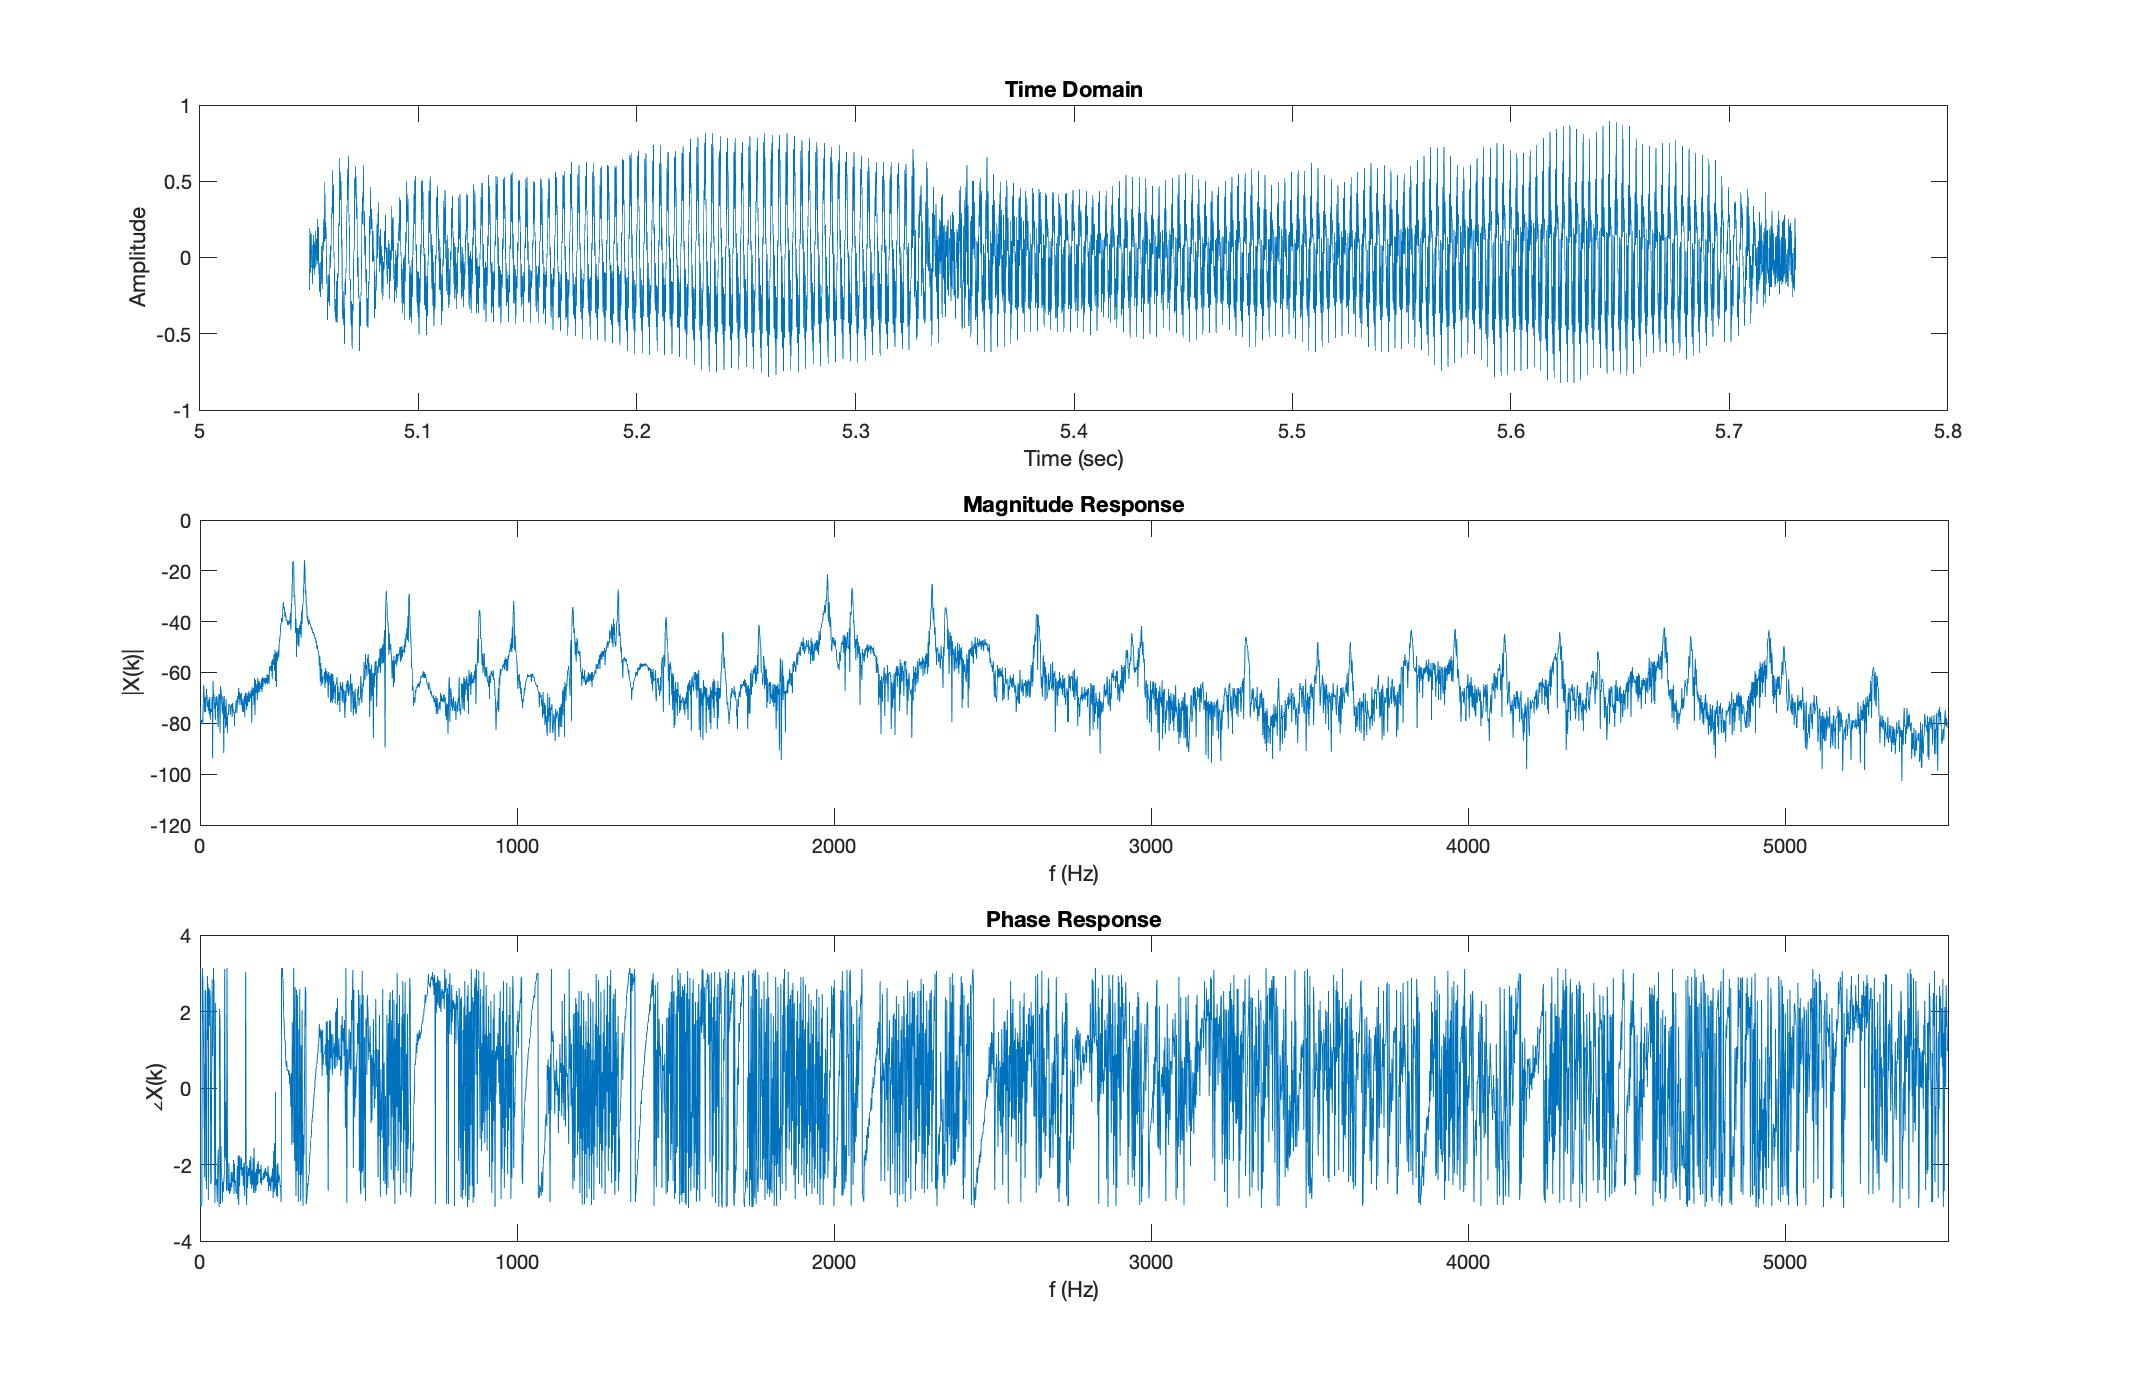
\includegraphics[scale = 0.22]{violinTwoNotes.jpg}
	\end{center}
\end{figure}

If we examine the magnitude response, we can see a set of two repeating peaks starting around 290Hz.  Using the
same intuitions from earlier, it would be logical to surmise that we have two notes playing with fundamentals around
290Hz and slightly higher at, say, 330Hz.  Though it is difficult to tell from Figure \ref{fig:violinTwoNotes}, those peaks
occur at exactly frequency bins 294Hz and 330.8Hz, both very close to the notes D4 and E4 respectively.  Indeed, it is
true that the violin plays those two notes from 5.05 to 5.75 seconds.  However, the magnitude spectrum fails
to indicate whether those notes are successive or simultaneous.  
The time domain, nevertheless, provides some clues.  We 
can see two distinct notes starting at 5.1 seconds and 5.35 seconds suggesting 
that the notes are played successively.  Choosing a large $N$ like 30000 in this example
unfortunately captured two distinct musical moments and merged the frequency content of both notes into one 
magnitude spectrum.  This is an example of where poor time resolution creates a confusing magnitude spectrum.  
A better
solution to this problem would be to use the DFT twice to analyze each note separately.  This would require smaller $N$,
and in turn our frequency resolution would be poorer.  One nice thing about $N = 30000$ though as shown in 
Figure \ref{fig:violinTwoNotes} is that the peak frequency bins are almost exactly the frequency of the original note,
making it easy to determine the fundamentals.  Reducing $N$ would potentially move the frequency bins farther away
from those fundamentals.  This is tradeoff we must make when choosing a size for $N$.  

As a general rule, if the audio file has a slow changing spectrum, choose a larger $N$.  The issues
related to time resolution will be mitigated if the audio experiences relatively little change in the time domain.  If the 
audio file has fast music or a rapidly changing spectrum, then use a smaller $N$.  Though the frequency resolution will be poorer, a larger $N$ will
simply capture too many musical events to parse.  
	\section*{The Inverse Fourier Transform and Spectral Processing}

\subsection*{The Inverse Discrete Fourier Transform}

We have seen how a time domain signal can be projected onto a basis of cosine and sine waves to give the
frequency domain representation of the sound.  Is it possible to inverse that process?  Can we take a signal
in the frequency domain and convert it to the time domain?  Fortunately, the answer is yes!  This technique
is called the Inverse Discrete Fourier Transform (abbreviated as IDFT).  Equation \ref{eq:idft} shows the equation
for the IDFT.  

\begin{equation}
	\label{eq:idft}
	x[n] = \frac{1}{N}\sum_{k = 0}^{N - 1}X_k \cdot e^{i\frac{2\pi}{N}kn}
\end{equation}

If we examine the IDFT, we can see that we sum the inner product of a complex sinusoids against all of our 
complex frequency bins $X_k$ to restore the original signal $x[n]$.  The equation for the IDFT is very similar
to the one for the DFT shown in Equation \ref{eq:dft}.  The only differences are $x[n]$ and $X_k$ are swapped,
the complex exponential is now positive, and the IDFT has a scaling constant of $\frac{1}{N}$.  The appendix
shows a proof that the IDFT and DFT are truly inverse operations.  The beauty of the IDFT is that it allows us
to convert back and forth between the frequency domain and the time domain.  We can convert a signal to the
frequency domain, perform some spectral manipulations and then convert back to the time domain, creating
a processed version of the original.  Though less frequently done, we could also build a signal in the frequency
domain and then use the IDFT to get the time domain representation of the sound.  At the end of the day, all 
signals need to be converted back to the time domain because all digital-to-analog converters (ADCs) require
time domain representations of sound.

\subsection*{Spectral Processing}

The DFT and IDFT provide the means to convert an audio signal to the frequency domain for processing and
then convert back to the time domain.  Spectral manipulation involves changing the complex numbers for
each $X_k$.  Simple operations include zeroing out bins, scaling the magnitude, changing the phase, rearranging
bins, etc.  There is a host of different techniques that one could apply.  One seemingly obvious example is
to create a brickwall filter by zeroing out frequency bins to create a high-pass, low-pass, or bandpass filter.
Zeroing out bins only creates a brickwall filter if the signal $x[n]$ is periodic along $N$.  Otherwise, nasty artifacts
will be present in the time domain once the IDFT is complete.  Discussing and analyzing various spectral 
techniques is beyond the scope of this guide; however, experimenting with simple spectral operations is good 
practice for developing intuitions.
	\section*{Beyond the DFT}

We have seen how the DFT can transform an audio signal into the frequency domain.  We have also
seen that it is not a perfect tool.  The DFT assumes two things:

\begin{enumerate}
	\item The signal $x[n]$ is periodic
	\item The $N$ samples constitute one period from $x[n]$
\end{enumerate}

We could add a third condition, namely that we should be careful to sample from a bandlimited signal so
that we do not produce aliasing in the frequency representation.  But generally this is assumed.  

Unfortunately, when these two main conditions are not obeyed, the DFT cannot accurately parse the frequency
components of $x[n]$.  Nearly all $x[n]$ in practice violate these two conditions.  Nevertheless we can look at
peaks in the magnitude spectrum to get a good estimate of where the original frequencies lie.  In general, the
magnitude spectrum contains the most important information we need. 

\subsection*{Short-Time Fourier Transform}

As we saw in the section on Time Resolution vs Frequency Resolution, too large of $N$ can blur 
different time components of the sound.  Generally we want to get a snapshot of the frequency domain at
any given moment.
The Short-Time Fourier Transform takes successive DFTs on a longer stretch of audio to get a sense of
how the frequency components of sound change over time.  In audio platforms like Max/MSP or SuperCollider
or underneath the hood in Digital Audio Workstations like Logic or ProTools, the Short-Time Fourier Transform
(abbreviated STFT) is the main tool we use for spectral processing.  We divide up an audio segment into
a series of small moments in time, take the DFT of each of those moments, and apply processing in the 
frequency domain to create some particular audio effect.  The STFT is also used for audio analysis.  We often
plot the results of the STFT as a spectrogram.  Figure \ref{fig:spectrogram} shows the spectrogram of an electric guitar.

The x-axis represents the time and the y-axis represents frequency.  Each vertical bar in the spectrogram 
represents one DFT of one segment of $N$ samples from the audio file.  The spectrogram plots the magnitude
response.  Higher magnitudes are distinguished from lower magnitudes using a color map.  In this 
spectrogram, the magnitude is charted on a decibel scale where higher magnitudes are brighter and lower magnitudes
are darker.  The spectrogram provides a nice visualization for how the frequency content of a sound evolves over
time.  

\begin{figure}[h]
	\caption{Spectrogram of strummed guitar chords}
	\label{fig:spectrogram}
	\begin{center}
		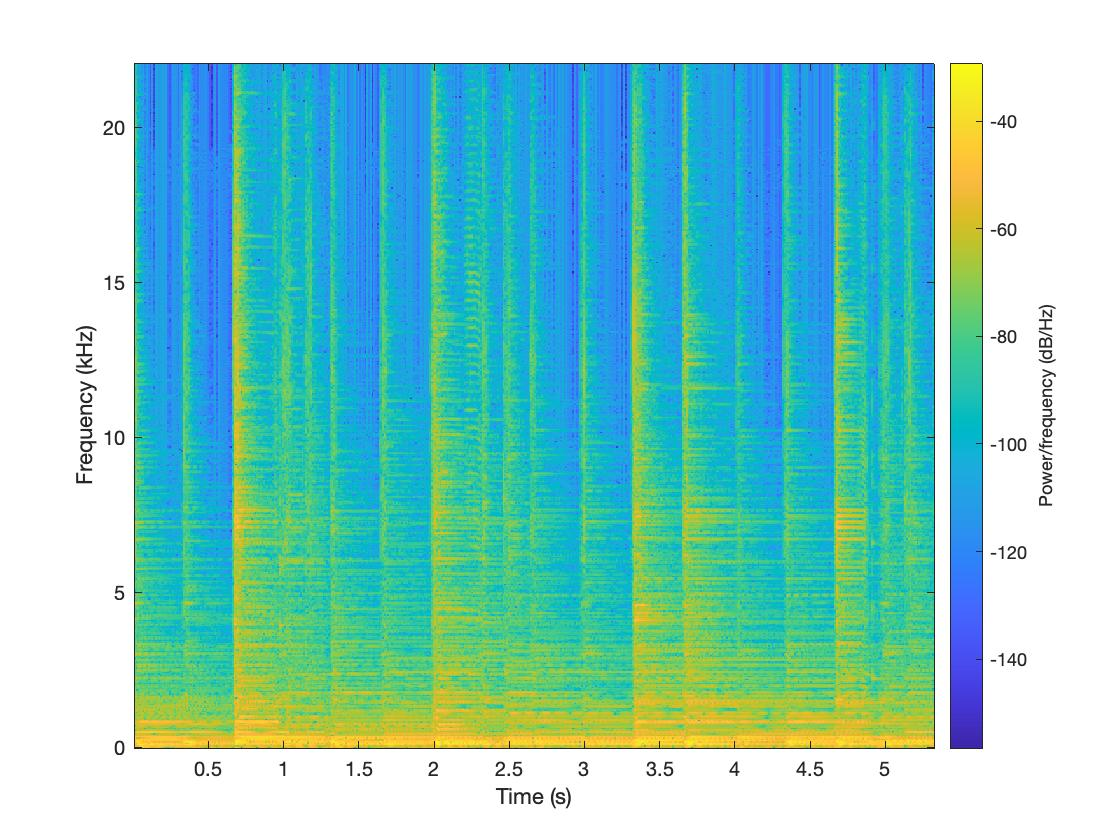
\includegraphics[scale = 0.35]{spectrogram.jpg}
	\end{center}
\end{figure}

In this spectrogram, it becomes easy to tell where each strum lies.  Like many instruments, the attack portion of
the guitar is percussive and noiser in sound.  Noise tends to have equal energy throughout the entire frequency 
spectrum.  In the spectrogram, those strums are the solid yellow and green vertical lines, representing equal
energy across that portion of audio.  The harmonic parts are the comb-like lines that protrude to the right
of those solid vertical lines.  In harmonic sounds, the frequency spectrum only has energy at the harmonics.
Those horizontal lines articulate the energy of each harmonic present in the sound.  Taken together, we can see
how the percussive attacks followed by the harmonic resonance gives a complete picture of the frequency
content for these guitar chords.

\subsection*{More DSP}

Understanding the tools of digital signal processing like the Discrete Fourier Transform is imperative for
audio programming and developing industry tools in audio.  For musicians, we care mostly about how to use
digital audio tools.  The actual 
implementation and mathematical framework 
necessary to understand DSP theory is left to programmers, audio technicians, and signal processing engineers.  Nevertheless, having a 
solid foundation in digital signal processing, and in particular the techniques to convert between
the time and frequency domains, will invariably make us better musicians and quicker to capitalize
on digital audio tools.  Hopefully, this guide has demystified the DFT to some degree and given you
better insight into this important tool for audio signal processing.
	\newpage
	%
	\section*{Appendix A - Review of Mathematical Concepts}

	\subsection*{Summation Notation}
	
	\subsection*{Complex Numbers}
 % math review
	%
	\section*{Appendix B - Proof of Orthogonality of Sinusoids}

	Here we prove the orthogonality of sinusoids both in discrete and continuous time.  We will start with continuous time since that is simpler to prove.  
	
	\subsection*{Orthogonality of Continuous Sinusoids}
	Let's first start with the claim that two sine waves that are periodic over the interval from 
	$[0, L]$ are orthogonal if their frequencies are different.  Let's call those two sine waves
	$\sin(\omega_1 t)$ and $ \sin(\omega_2 t )$.  $\omega$ is angular frequency and can
	be easily converted to frequency using the equation $\omega = 2\pi f$.  We use $\omega$ here because it makes the
	math a little cleaner and more concise.  Recall that orthogonality is the sum of pointwise products.  We
	can use an integral to express the summation.  An integral is simply the sum of some function over every point 
	between some lower bound and some upper bound.  Here we want that the function to be the product of our two
	functions.  Therefore, we can express the orthogonality of these two arbitrary sinusoids as such:
	
	\begin{equation}
		\label{eq:ip}
		\int_{0}^{L}\sin(\omega_1 t)\sin(\omega_2 t)dt
	\end{equation}
	
	If you work through the calculus, you will find the following solution to the integral:
	
	\begin{equation}
		\frac{1}{2}\left(\frac{\sin((\omega_1 - \omega_2)L)}{\omega_1 - \omega_2} - \frac{\sin((\omega_1 + \omega_2)L)}{\omega_1 + \omega_2}\right)
		\label{eq:orth}
	\end{equation}
	
	To prove orthogonality, we need to go back to our original assumption about periodicity.  We assumed that 
	both sinusoids were periodic along the interval 0 to $L$.  How can we express that mathematically?  Any periodic
	sinusoid along $L$ must complete an integer number of cycles.  Let's call that integer number of cycles $n$.  
	We can now express the frequency of such a sinusoid as $n/L$.  This should make intuitive sense.  For
	example, a 50Hz sine wave completes 50 periods of a sine wave in one second, equivalent to $n = 50$ and $L = 1$.
	So we can always think of the frequency of a sinusoid as some number of cycles divided by some unit of time.  
	Finally, if $f = n/L$ and $\omega = 2\pi f$, we can combine those two equations to say 
	
	\begin{equation}
		\label{eq:period}
		\omega = 2\pi n/L
	\end{equation}
	
	Now consider the two sine expressions in equation (\ref{eq:orth}): $\sin((\omega_1 - \omega_2)L)$ and 
	$\sin((\omega_1 + \omega_2)L)$.  Let's now replace $\omega_1$ and $\omega_2$ with our result from equation
	(\ref{eq:period}).  We can see that $\sin((\omega_1 - \omega_2)L) = \sin(2\pi(n_1 - n_2))$ and 
	$\sin((\omega_1 + \omega_2)L) = \sin(2\pi(n_1 + n_2))$.  Here is where our assumption pays off.  Remember
	that $n_1$ and $n_2$ represent the number of cycles each of the two arbitrary sinusoids completes in time $L$.
	Furthermore, recall that $n_1$ and $n_2$ are whole numbers because in order for the sinusoids to be periodic, 
	they must have completed a whole number of cycles (i.e., no partial cycles).  Therefore, $n_1 + n_2$ and $n_1 - n_2$ 
	must also be whole numbers because adding or subtracting whole numbers from each other always yields whole
	numbers.  And finally, since $\sin$ is always zero at multiples of $2\pi$, we can see that $\sin(2\pi(n_1 + n_2))$
	and $\sin(2\pi(n_1 - n_2))$ are always zero.  Thus equation (\ref{eq:orth}) is always zero when $\omega_1 \neq
	\omega_2$.  This proves orthogonality when two sine waves have different frequencies yet are periodic along the
	same time span.  
	
	One final thing to consider is what happens when the frequencies are the same (i.e., $\omega_1 = \omega_2$).  We
	actually cannot tell based on equation (\ref{eq:orth}) because that equation is undefined when 
	$\omega_1 = \omega_2$.  However, we can go back to our original integral from equation (\ref{eq:ip}) and solve
	knowing that $\omega_1 = \omega_2$.  
	
	\begin{equation}
	\int_{0}^{L}\sin(\omega_1 t)\sin(\omega_2 t)dt = \int_{0}^{L}\sin^2(\omega_1 t)dt = \frac{L}{2} - \frac{\sin(2\omega_1 L)}{4 L}
	\end{equation}
	
	By our similar logic above, we can show that $\sin(2\omega_1 L)$ is always zero leaving our result to be just
	$L/2$.  It's crucial to note that when $\omega_1 = \omega_2$ that the two sine waves are \textbf{not} orthogonal
	because their inner product yields a non-zero result.
	
	We can follow the same script as above to show similarly that the inner product of a sine wave and a cosine wave
	or two cosine waves are orthogonal at different frequencies. \footnote{Intererstingly, the inner product of two cosine
	waves of the same frequency will yield a non-zero result just like the inner product of two sine waves.  However, the 
	inner product of a cosine wave and a sine wave is always zero even if the frequencies are the same.  Thus, periodic 
	sine and cosine waves are always orthogonal.  It turns out that any two periodic sinusoids are orthogonal if separated
	by a phase of $\pi/2$.}  Again,
	we must make the same assumption that the waves are periodic along some time interval which we call $L$.  Notice
	that this is essential for the proof to work because we had to be able to state that $n_1$ and $n_2$ were integers.
	If we could not assert that fact, we could not say that $\sin(2\pi(n_1 + n_2))$
	and $\sin(2\pi(n_1 - n_2))$ are always zero.
	
	Before we move to analyzing discrete sinusoids, it should be noted that sinusoids of different frequencies are 
	orthogonal regardless of their phase or amplitude.  To show that we need to say that the following always yields
	zero when $\omega_1 \neq \omega_2$
	
	\begin{equation}
	\label{eq:generalorth}
	\int_{0}^{L}A_1\sin(\omega_1 t + \phi_1)A_2\sin(\omega_2 t + \phi_2)dt
	\end{equation}
	
	It is actually quite simple to show this using what we have established so far using trigonometric identities.  Here
	we will need the identity that $\sin(u + v) = \sin(u)\cos(v) + \cos(u)\cos(v)$.  If we apply the identity to each 
	sine wave in equation (\ref{eq:generalorth}), we get the following:
	
	$$ 
	A_1A_2\int_{0}^{L}\left[\sin(\omega_1 t)\cos(\phi_1) + \cos(\omega_1t)\sin(\phi_1)\right]
	\left[\sin(\omega_2 t)\cos(\phi_2) + \cos(\omega_2t)\sin(\phi_2)\right]dt
	$$	
	
	After some unexciting multiplication and simplification, we can reduce our expression down to the following sum:
	
	\begin{equation}
	\begin{split}
		A_1A_2\cos(\phi_1)\cos(\phi_2)\int_{0}^{L}\sin(\omega_1)\sin(\omega_2)dt \; &+ \\
A_1A_2\cos(\phi_1)\sin(\phi_2)\int_{0}^{L}\sin(\omega_1)\cos(\omega_2)dt \; &+ \\
A_1A_2\sin(\phi_1)\cos(\phi_2)\int_{0}^{L}\cos(\omega_1)\sin(\omega_2)dt \; &+ \\
A_1A_2\sin(\phi_1)\sin(\phi_2)\int_{0}^{L}\cos(\omega_1)\cos(\omega_2)dt
	\end{split}
	\end{equation}

	We just showed that each one of these integrals is equal to zero when $\omega_1 \neq \omega_2$.  Therefore,
	two periodic sinusoids are always othrogonal when their frequencies are different regardless of phase or amplitude.
	
	\subsection*{Orthogonality for Sampled Sinusoids}
	We have exhaustively shown the relationship between periodicity, frequency and orthogonality for continuous 
	sinusoids.  But we can't just assume the same relationships are true when we sample sinusoids.  As it turns out,
	it is indeed true that the same relationships hold but let us walk through a bit of the logic to see how we can arrive
	at a similar conclusion.
	
	Sampling of any signal occurs at some regular interval which we will call $T$.  That interval is related to sampling
	rate (usually denoted $f_s$) by the equation $T = 1/f_s$.  This should make intuitive sense.  As the sampling rate
	increases, the sampling period $T$ should get smaller and smaller because we need to take more and more samples
	for the same duration of time.  We can also figure out the time $t$ of sample number $n$ by simply writing 
	$t = nT$.  Therefore we can get any sample number $n$ from some continuous sinusoid by writing 
	$A\sin(2\pi f nT + \phi)$ where $t$ is replaced by $nT$.  
	
	Orthogonality for sampled sinusoids is like orthogonality for vectors.  We take the product for each sample of
	the two sinusoids and sum them together.  Mathematically, we can use summation notation to express that.  Let's
	assume that we have two sine waves that are periodic from time 0 to $L$.  We will take $N$ samples from each of
	the two sinusoids with sample number $n = 0$ corresponding to time $t = 0$.  Because these two sinusoids are
	periodic from 0 to $L$, we know that they complete integer number of cycles.  Let's call the total number of cycles
	they complete $k_1$ and $k_2$.  The frequency then for each of those two sinusoids will be $f_1 = k_1/L$ and
	$f_2 = k_2/L$.  Here is the expression for our inner product:
	
	\begin{equation}
		\label{eq:orthDiscrete}
		\sum_{n = 0}^{N-1}\sin(2\pi f_1Tn)\sin(2\pi f_2Tn)
	\end{equation}
	
	Note that our summation runs from 0 to $N-1$ and not $N$ because the 0th sample is part of our total number of
	samples.  So we are in fact taking a total of $N$ samples.
	
	Using the identity $\sin(u + v) = \sin(u)\cos(v) + \cos(u)\cos(v)$, let's divide the summation into two parts:
	
	$$\frac{1}{2}\sum_{n = 0}^{N-1}\cos(2\pi (f_1 - f_2)Tn) - \frac{1}{2}\sum_{n = 0}^{N-1}\cos(2\pi (f_1 + f_2)Tn)$$
	
	It doesn't seem that will be able to take the discrete sum over a cosine wave but there is acutally an identity that
	will help us.  The proof for the identity is rather clever and requires complex numbers.  We won't go through it here
	but the identity is below:
	
	\begin{equation}
		\label{eq:sumCos}
		\sum_{n=0}^{N - 1}\cos(2\pi fn) = \frac{\cos(\pi f(N - 1))\sin(\pi fN)}{\sin(\pi f)}
	\end{equation}
	
	We can subsitute $(f_1 - f_2)T$ and $(f_1 + f_2)T$ for $f$ from equation (\ref{eq:sumCos}) and to get
	
	\begin{equation}
	\label{eq:noSumDiscrete}
	\frac{1}{2}\left[ \frac{\cos(\pi (f_1 - f_2)T(N - 1))\sin(\pi (f_1 - f_2)TN)}{\sin(\pi (f_1 - f_2)T)} - \frac{\cos(\pi (f_1 + f_2)T(N - 1))\sin(\pi (f_1 + f_2)TN)}{\sin(\pi (f_1 + f_2)T)}\right]
	\end{equation}
	
	Equation (\ref{eq:noSumDiscrete}) looks like a giant mess but let's take a careful look at $\sin(\pi (f_1 - f_2)TN)$
	and $\sin(\pi (f_1 + f_2)TN)$.  Both can be simplified.  We know $f_1 = k_1/L$ and $f_2 = k_2/L$.  We also
	know that the sample rate $f_o$ is equal to the number of samples per second which is equivalent to the total
	number of samples divided by the total time, or simply $N/L$.  Since $T = 1/f_o$, then we can also say that 
	$T = L/N$.  Now let's reduce $\sin(\pi (f_1 - f_2)TN)$.
	
	$$\sin(\pi (f_1 - f_2)TN) = \sin(\pi (\frac{k_1}{L} - \frac{k_2}{L})\frac{L}{N}N) = \sin(\pi(k_1 - k_2))$$
	
	Recall that $k_1$ and $k_2$ are integers.  Just as we saw with continuous sinusoids, we can see that sine will 
	always be zero because any integer multiple of $\pi$ for sine is always zero.  The same will be true 
	$\sin(\pi (f_1 + f_2)TN) = \sin(\pi (f_1 + f_2))$.  Therefore, we can conclude that when $f_1 \neq f_2$ our 
	expression from equation (\ref{eq:sumCos}) will always be zero.  Hence, our two sinusoids are always orthogonal
	at different frequencies.  We do need to be a little careful here.  We have to be sure that neither of the
	denominators in equation (\ref{eq:noSumDiscrete}) are zero.  Otherwise, we cannot make the claim of
	orthogonality because the equation would be undefined.  Fortunately, it should not be an issue in any 
	practical application.  We need to be concerned when $f_1/f_o - f_2/f_o$ or $f_1/f_o + f_2/f_o$ is an
	integer.  But that can only happen if the frequencies $f_1$ and $f_2$ are the same or if $f_1$ and $f_2$ 
	exceed the Nyquist frequency of $f_o/2$.  In the former case, we are not making any claims yet about
	when the frequencies are the same.  In the latter case, any practical digital signal should have frequencies
	at or above the Nyquist frequency properly removed by anti-aliasing filtering.  
	
	Similar to the continuous case, our equation (\ref{eq:noSumDiscrete}) cannot tell us anything about 
	when $f_1$ equals
	$f_2$ because it is undefined at that point.  We need to go back to the original summation from equation 
	(\ref{eq:orthDiscrete}) and set $f_1 = f_2$.  
	
	\begin{equation}
	\label{eq:sameFreqOrth}
	\sum_{n = 0}^{N-1}\sin^2(2\pi f_1Tn) =
	 \frac{1}{2}\sum_{n = 0}^{N-1}1 - \frac{1}{2}\sum_{n = 0}^{N-1}\cos(4\pi f_1Tn) = 
	 \frac{N}{2} - \frac{1}{2}\sum_{n = 0}^{N-1}\cos(2\pi (\frac{2f_1}{f_o})n)
	\end{equation}
	
	The final summation after simplification from equation (\ref{eq:sameFreqOrth}) can equal at most $N/2$ when
	cosine is equal to 1.  Only then when $f_1 = f_2$ will we get orthogonality.  At any other point the equation
	will be non-zero.  If we look at the summation, we will see that cosine equals 1 only when $f_1 = f_2 = 0$ or 
	when $f_1 = f_2 = f_o/2$ (i.e., the Nyquist frequency).
	
	\textbf{Might be nice to add about what happens with cos * cos and sin * cos}
	
	\subsection*{Some final thoughts on orthogonality}
		The great power of orthogonality is to test whether some sine wave of unknown frequency $f_{unknown}$
	is equal to some frequency $f_{test}$ which we do know.  The section on ... deals with the importance of this 
	issue.  Orthogonality is our tool to determine if $f_{unkown}$ equals $f_{test}$.  If you take the inner product
	of both $f_{unknown}$ and $f_{test}$ when they are continuous, a non-zero inner product confirms with
	certainty that they are two sinusoids of the same frequency.  The same is true in the discrete case as well.
	However, if you take the inner product and $f_{unknown}$ and $f_{test}$ are orthogonal, you do \textbf{not}
	know with certainty if the two sinusoids have different frequencies.  The section on ... illustrates that sinusoids
	separated by a phase of $\pi/2$ are orthogonal even if they have the same frequency.  But note that in the
	discrete case, you can sometimes achieve orthogonality for the same sinusoids if the frequencies are both zero 
	or the Nyquist frequency, regardless of phase.  We generally do not care too much about the frequency 
	components at DC (i.e., when $f_{unknown}$ = 0) because we hopefully have removed most DC bias from
	our signal.  Likewise, we do not often care about the Nyquist frequency because any good audio signal will
	have removed frequencies at or above the Nyquist frequency with some sort of anti-aliasing filter.  So
	in practice, we should not have to worry about such potential issues but its pivotal to understand the math
	so we can understand exactly what our tools can and cannot do.
 % proof of orthogonality
	%\section*{Appendix C: Inverse DFT Stuff}

In this appendix, we will show that the IDFT can be used to recover the original signal $x[n]$ from the
frequency domain.  Recall Equations \ref{eq:dft} and \ref{eq:idft} for the DFT and IDFT, respectively.  Let's
start the equation for the IDFT shown below:

$$ x[n] = \frac{1}{N}\sum_{k = 0}^{N - 1} X_k e^{i\frac{2\pi}{N}kn}$$

We want to show that the right side is also $x[n]$ if $X_k$ was calculated using the DFT on $x[n]$.  Here,
we can substitute in the DFT equation for $X_k$ on the sequence $x[n]$.  For clarity, we will use a different
index variable $m$ for the DFT equation to distinguish it from the IDFT index variable $n$.

$$ x[n] = \frac{1}{N}\sum_{k = 0}^{N - 1} \bigg(\sum_{m = 0}^{N - 1}x[m] \cdot e^{-i\frac{2\pi}{N}km} \bigg) e^{i\frac{2\pi}{N}kn}$$

Here we will do some clever rearranging.

$$x[n] = \frac{1}{N}\sum_{k = 0}^{N - 1} \sum_{m = 0}^{N - 1}x[m] \cdot e^{i\frac{2\pi}{N}k(n - m)} $$

$$x[n] = \frac{1}{N}\sum_{m = 0}^{N - 1} \sum_{k = 0}^{N - 1}x[m] \cdot e^{i\frac{2\pi}{N}k(n - m)} $$

Note that the switching of summations is a clever trick that occurs all the time in DFT proofs.

$$x[n] = \sum_{m = 0}^{N - 1} \frac{1}{N}\sum_{k = 0}^{N - 1}x[m] \cdot e^{i\frac{2\pi}{N}k(n - m)} $$

$$x[n] = \sum_{m = 0}^{N - 1} x[m] \bigg(\frac{1}{N}\sum_{k = 0}^{N - 1} e^{i\frac{2\pi}{N}k(n - m)} \bigg)$$

Let us now analyze the portion in parentheses.  If $n \neq m$, then $\frac{1}{N}\sum_{k = 0}^{N - 1}
 e^{i\frac{2\pi}{N}k(n - m)} = \frac{1 - e^{2\pi i (n -m)}}{N(1 - e^{2\pi i (n -m)/N})} = 0$.  The trick here is
 solving the summation using the formula for a finite geometric sum.  We can reason that the number is always
 zero because $n - m$ is always an integer and therefore the complex exponential has a phase that is always
 a multiple of $2\pi$.  If $n = m$, then $\frac{1}{N}\sum_{k = 0}^{N - 1} e^{i\frac{2\pi}{N}k(n - m)} = \frac{1}{N}\sum_{k = 0}^{N - 1}1 = \frac{N}{N} = 1$.  
 
 If we analyze the outer summation, then we will see that each term in the summation will be 0 except when
 $n = m$.  That term has a value of $x[m]$ or $x[n]$.  Therefore, we have showed that the right side does
 indeed reduce to $x[n]$.   % proof of inverse transform
\end{document}